\chapter[Langages de l'informatique]{Langages de l'informatique}% Langages de l'informatique
\label{chap:VI}

\lettrine{L}{a programmation est une des activités les plus visibles} de l'informatique. En amont, avant de se lancer tête baissée dans l'apprentissage d'un langage de programmation et le codage, il est souvent utile de détailler le mode d'emploi ou la recette permettant d'aboutir au résultat voulu indépendamment de toute programmation effective : cette étape est couverte par ce qu'on appelle l'algorithmique.

Ensuite, le terrain étant balisé, il devient plus aisé\parnote{De nos jours, on utilise également des outils de modélisation comme UML --- \textup{Unified Modeling Language} --- et autres processus de codage comme les méthodes dites agiles qui facilitent la conception et le développement des programmes informatiques, surtout pour les applications volumineuses impliquant de multiples contributeurs.} de s'atteler à la programmation en tant que telle à l'aide d'un langage choisi en fonction de multiples critères contextuels et pragmatiques. Ce chapitre aborde ces deux facettes du traitement de l'information et de l'expression entre humain et machine.
\parnotes

\vspace{1.5\baselineskip}

%----------
\section[Algorithmique]{Algorithmique}
\label{sec:VI.1}

L'algorithmique est la science des algorithmes, mot dérivé du nom du mathématicien Muhammad \textsc{al-Khwarizmi} ayant vécu au IX\frup{e} siècle.

Aujourd'hui, il s'agit d'établir, au moyen d'un langage quasiment naturel et de concepts élémentaires, une suite d'instructions que la machine est à même de « comprendre » et d'exécuter.

\subsection[Notions fondamentales]{Notions fondamentales}
\label{sub:VI.1.1}

Un algorithme répond au double objectif de conduire à un résultat, si possible correct, en un nombre fini d'opérations. Par définition, il prend un ensemble de données en entrée, exprime un traitement spécifique et fournit des données en sortie.

\subsubsection[Décomposition en tâches]{Décomposition en tâches}
\label{subsub:VI.1.1.1}

\begin{marginvideo}
	[\label{vid:VI.1}Décomposition en tâches.]%
	\movie[width=\marginparwidth,showcontrols]%
		{
\includegraphics[width=\marginparwidth]{./Images/Pictograms/film-strip-dark-electric-blue.png}}%
		{./Videos/Chapter06/vidVI-01-algorithmique-tasks-HD.mp4}%
	\launchvideo{./Videos/Chapter06/vidVI-01-algorithmique-tasks-HD.mp4}
\end{marginvideo}

À l'instar des champs disciplinaires de la physique, il est souvent impossible de résoudre directement des problèmes complexes. La démarche est alors de décomposer la problématique \nopagebreak en éléments simples auxquels on sait répondre et d'apporter petit-à-petit les briques manquantes menant à la solution. 
Cette approche est identique en algorithmique, où l'obtention d'une solution ne peut s'envisager que par étapes successives du fait que l'ordinateur ne sait manipuler qu'un nombre limité de concepts et d'instructions.

Pour expliciter le propos, on considère un algorithme conduisant à savoir si des élèves ont obtenu la moyenne à une épreuve corrigée. Autrement dit, étant donné un tableau de notes potentiellement grand, déterminer combien d'élèves ont la moyenne.

\vspace{-0.5\baselineskip}
\begin{center}
\begin{tikzpicture}[start chain=1 going {right=of \tikzchainprevious.east},
                    node distance=-\pgflinewidth, every node/.style={draw}]
\node [on chain, minimum width=10mm] {\strut $8$};
\node [on chain, minimum width=10mm] {\strut $12$};
\node [on chain, minimum width=10mm] {\strut $20$};
\node [on chain, minimum width=10mm] {\strut $\num{16.5}$};
\node [on chain, minimum width=10mm] {\strut $11$};
\node [on chain, minimum width=10mm] {\strut $\num{8.5}$};
\node [on chain, minimum width=10mm] {\strut $3$};
\node [on chain, minimum width=10mm] {\strut $16$};
\node [on chain, minimum width=10mm] {\strut $\num{10.5}$};
\end{tikzpicture}

\begin{tikzpicture}[start chain=1 going {right=of \tikzchainprevious.east},
                    node distance=-\pgflinewidth, every node/.style={draw}]
\node [on chain, minimum width=10mm] {\strut $8$};
\node [on chain, minimum width=10mm, fill=firstcolor] {\strut\textcolor{white}{$12$}};
\node [on chain, minimum width=10mm, fill=firstcolor] {\strut\textcolor{white}{$20$}};
\node [on chain, minimum width=10mm, fill=firstcolor] {\strut\textcolor{white}{$\num{16.5}$}};
\node [on chain, minimum width=10mm, fill=firstcolor] {\strut\textcolor{white}{$11$}};
\node [on chain, minimum width=10mm] {\strut$\num{8.5}$};
\node [on chain, minimum width=10mm] {\strut $3$};
\node [on chain, minimum width=10mm, fill=firstcolor] {\strut\textcolor{white}{$16$}};
\node [on chain, minimum width=10mm, fill=firstcolor] {\strut\textcolor{white}{$\num{10.5}$}};
\end{tikzpicture}
\end{center}
\vspace{-0.5\baselineskip}

Pour le tableau ci dessus, c'est assez facile car on peut compter les notes au dessus de la moyenne « à la main », mais pour d'autres cas de figure avec plusieurs centaines de notes, l'ordinateur est un secours.

\sidegraphic{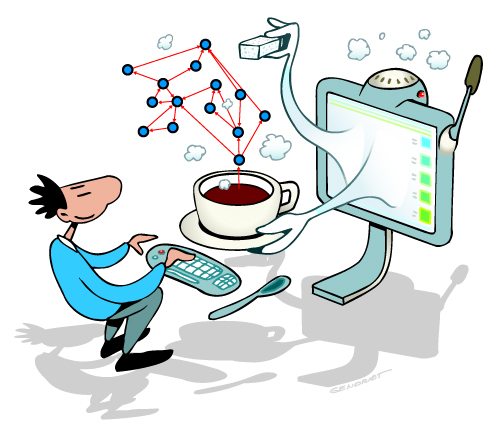
\includegraphics[width=\linewidth]{grahVI-01-ingredients-algo-paul-gendrot-interstices.jpg}}{Paul Gendrot}%
La question est alors de savoir ce que sait faire un ordinateur. Il peut réaliser des tâches simples et unitaires comme :
\begin{itemize}
\item faire un calcul ;
\item mettre le résultat du calcul dans une variable ;
\item exécuter séquentiellement (l'une après l'autre) des tâches ;
\item conduire un test pour choisir quelle tâche exécuter ensuite ;
\item faire une boucle (tant que quelque chose ne se passe pas)...
\end{itemize}

Reconsidérons le tableau de notes précédent et supposons qu'il ait un million de cases. Il est indubitablement nécessaire de réagir autrement qu'en comptant à la main. 

En isolant une case, on la regarde et si son contenu est plus grand que $10$ on renvoie $1$, sinon $0$. Si le tableau contient $n$ cases avec $n > 1$, supposons que l'on sait que sur les $n-1$ cases premières cases, on a $s$ élèves qui ont la moyenne alors, en observant la n-ième case, si son contenu est plus grand que $10$, il y a $s+1$ élèves ayant la moyenne, sinon il y en a $s$. Dès lors, on peut transcrire la problématique en algorithme exprimé en pseudocode.

\begin{algorithm}{Notes supérieures à 10}
Variable n entier > 0
Tableau  t taille n §(valeurs de t[0] à t[n-1])§
Variable s entier > 0

s §$\leftarrow$§ 0
Pour i allant_de 0 à n-1, Faire
  Si (t[i] ≥ 10)
    Alors s §$\leftarrow$§ s + 1
  FinSi
FinPour
\end{algorithm}

\begin{gofurther}
\lightbf{Formation complémentaire}
\begin{itemize}\jazzitem
	\item Partie 1.1 et 1.4 du \href{https://pixees.fr/classcode/formations/module1/\#partie1}{\#1 Module fondamental : découvrir la programmation créative}, \textsc{Class´Code}. Cette formation pour enseignants du secondaire offre des vidéos accessibles en cliquant sur le pictogramme \faIcon[regular]{play-circle} --- NB: \textsc{Scratch} n'est pas au programme SNT, mais les élèves ont maintenant été formés à \textsc{Scratch} en collège ou primaire ; cette ressource permet de se mettre à niveau par rapport à cette compétence.
\end{itemize}

\lightbf{Articles}
\begin{itemize}\jazzitem
\item \href{https://fr.wikipedia.org/wiki/Assembleur}{Le langage assembleur}, Wikipedia ;
\item \href{https://interstices.info/les-ingredients-des-algorithmes/}{Les ingrédients des algorithmes}, Gilles \textsc{Dowek}, Thierry \textsc{Viéville}, Jean-Pierre \textsc{Archambault}, Emmanuel \textsc{Baccelli} et Benjamin \textsc{Wack}, \textsc{Interstices}, 21 avril 2010.
\end{itemize}

\lightbf{Vidéo}
\begin{itemize}\jazzitem
\item \href{https://www.youtube.com/watch?v=AWsNFN0GCuQ}{Class'Code Didacticiel - D-Clics numérique}, initiation à la notion d'algorithme à travers la métaphore culinaire usuelle par Thierry Viéville, YouTube, (8mn 35s), 2016.
\end{itemize}
\end{gofurther}

\subsubsection[Variables]{Variables}
\label{subsub:VI.1.1.2}

\begin{marginvideo}
	[\label{vid:VI.2}Variables.]%
	\movie[width=\marginparwidth,showcontrols]%
		{
\includegraphics[width=\marginparwidth]{./Images/Pictograms/film-strip-dark-electric-blue.png}}%
		{./Videos/Chapter06/vidVI-02-algorithmique-variables-HD.mp4}%
	\launchvideo{./Videos/Chapter06/vidVI-02-algorithmique-variables-HD.mp4}
\end{marginvideo}

Qu'est-ce qu'une variable ? C'est un espace mémoire soit locale, soit distante, où le programme stocke une valeur ou une structure de donnée compliquée. Une variable est censée changer au cours de l'exécution du programme, sinon on parle plutôt de constante.

On peut citer quelques exemples de variables comme :
\begin{itemize}
\item  le nombre de \textit{followers}, de vues d'une vidéo sur \textsc{YouTube}, de \textit{like}, etc. (un entier) ;
\item la moyenne d'un élève (un réel, nombre à virgule flottante) ;
\item toutes les notes d'une classe (un tableau, un tableau de tableaux, une base de données) ;
\item mais encore d'autres données plus complexes, à savoir une table de hachage, une liste doublement chaînée, etc.
\end{itemize}

Différentes manipulations sur les variables sont possibles :
\begin{itemize}
\item elle doit être créée (cela dépend en fait du langage de programmation, certains déclarant la variable lors de leur utilisation) ;
\item elle peut être affectée d'une valeur particulière (\texttt{i $\leftarrow$ 0}) ;
\item elle peut être modifiée d'une valeur particulière (\texttt{i $\leftarrow$ i+1}) ;
\item elle peut être l'entrée du programme.
\end{itemize}

Les variables sont souvent typées, c'est-à-dire qu'en les déclarant on leur attribue une catégorie connue. On distingue à cet effet :

\begin{multicols}{2}
\begin{itemize}
\item les entiers ;
\item les chaînes de caractères ;
\item les nombres flottants ;
\item les tableaux ;
\item les pointeurs ;
\item les structures composées...
\end{itemize}
\end{multicols}

\begin{gofurther}
\lightbf{Formation complémentaire}
\begin{itemize}\jazzitem
	\item Partie 3 du \href{https://pixees.fr/classcode/formations/module1/\#partie3}{\#1 Module fondamental : découvrir la programmation créative}, \textsc{Class´Code}. Cette formation pour enseignants du secondaire offre des vidéos accessibles en cliquant sur le pictogramme \faIcon[regular]{play-circle}.
\end{itemize}

\lightbf{Articles}
\begin{itemize}\jazzitem
\item \href{https://fr.wikipedia.org/wiki/Variable_(informatique)}{Les variables}, Wikipedia ;
\item \href{https://fr.wikipedia.org/wiki/Pointeur_(programmation)}{Les pointeurs}, Wikipedia ;
\item \href{https://interstices.info/naissance-des-langages-de-programmation/}{Naissance des langages de programmation}, Sacha \textsc{Krakowiak} et Jacques \textsc{Mossière}, \textsc{Interstices}, 24 janvier 2012.
\end{itemize}

\lightbf{Vidéo}
\begin{itemize}\jazzitem
\item \href{https://www.youtube.com/watch?v=zbpo7XB5bTo&index=7&list=PLWvGMqXvyJAPWRbAADvvxsWUtiRZ_dGqT}{La notion de variable selon Gilles Dowek}, (présentation très large public de la notion de variable, en 50 secondes par Thierry \textsc{Viéville}), YouTube.
\end{itemize}
\end{gofurther}

\subsubsection[Instructions élémentaires]{Instructions élémentaires}
\label{subsub:VI.1.1.3}

\begin{marginvideo}
	[\label{vid:VI.3}Instructions élémentaires.]%
	\movie[width=\marginparwidth,showcontrols]%
		{
\includegraphics[width=\marginparwidth]{./Images/Pictograms/film-strip-dark-electric-blue.png}}%
		{./Videos/Chapter06/vidVI-03-algorithmique-instructions-HD.mp4}%
	\launchvideo{./Videos/Chapter06/vidVI-03-algorithmique-instructions-HD.mp4}
\end{marginvideo}

Le cœur de l'algorithmique est dérivé des instructions élémentaires qu'il est possible de réaliser avec un ordinateur. Comme pour l'ADN des cellules du monde vivant, elles sont au nombre de quatre à partir desquelles on peut élaborer \emph{n'importe quel algorithme}.

La première instruction est l'affectation déjà évoquée précédemment ; à une variable on associe une valeur donnée : \texttt{i $\leftarrow$ 17}, \texttt{i $\leftarrow$ i+1}.

La deuxième instruction est le test :

\vspace{-0.7\baselineskip}
\begin{center}
\lstinline[style=lstalgostyle,basicstyle=\normalsize\shellttfont]{Si <booléen> Alors <instruction> Sinon <instruction>}.
\end{center}
\vspace{-0.7\baselineskip}

Si une valeur booléenne est vraie --- une expression booléenne retourne soit vrai, soit faux ---, alors on exécute une instruction, sinon on exécute une autre instruction.

Quelques exemples de tests sont donnée par :
\begin{itemize}
\item une valeur est-elle supérieure à 10 ?
\item un calcul risque-t-il de dépasser les valeurs maximales/minimales du type de la variable ?
\item est-il possible de déborder des limites licites d'un tableau ?
\end{itemize}

L'instruction suivante est la séquence. L'intérêt de l'informatique est d'exécuter un certain nombre d'opération les unes après les autres

\vspace{-0.7\baselineskip}
\begin{center}
\lstinline[style=lstalgostyle,basicstyle=\normalsize\shellttfont]{<instruction> ; <instruction>}.
\end{center}
\vspace{-0.7\baselineskip}

On peut en fournir quelques exemples :
\begin{itemize}
\item affectation puis test ;
\item affectation, puis boucle, puis test ;
\item affectation, puis affectation, puis affectation, puis affectation.
\end{itemize}

Enfin, la dernière instruction est la boucle. On en distingue deux formulation : la boucle « \texttt{Pour} » et la boucle « \texttt{Tant que} ».

\vspace{-0.7\baselineskip}
\begin{center}
\lstinline[style=lstalgostyle,basicstyle=\normalsize\shellttfont]{Pour variable de valeur à valeur Faire <instruction> FinPour}.
\end{center}
\vspace{-0.7\baselineskip}

La boucle « \texttt{Pour} » sert par exemple à parcourir un tableau pour en extraire des données ou mener des calculs : chercher un maximum, calculer une moyenne, remplir un tableau, etc.

\vspace{-0.7\baselineskip}
\begin{center}
\lstinline[style=lstalgostyle,basicstyle=\normalsize\shellttfont]{TantQue booléen Faire <instruction> FinTantQue}.
\end{center}
\vspace{-0.7\baselineskip}

La boucle « \texttt{TantQue} » est plus générale et permet de réaliser plus de choses que la boucle « \texttt{Pour} », mais nécessite plus d'attention notamment au niveau de son instruction. Il faut en effet être sûr que le programme s'arrête et qu'une boucle infinie ne s'installe. On parle de problème de terminaison.

Une des utilisations traditionnelles de la boucle « \texttt{TantQue} » est une suite convergente qui va calculer par itération successives les valeurs, jusqu'à ce quelles soient suffisamment proches.

Soit comme exemple applicatif, un algorithme de recherche par dichotomie d'une valeur dans un tableau \emph{trié}. En sortie, on obtient un booléen qui renvoie si la valeur est dans le tableau ou non.
\begin{algorithm}{Recherche dichotomique}
Variable n entier > 0
Tableau  t taille n // tableau trié
Variable v, sup, inf entier

inf §$\leftarrow$§ 0;
sup §$\leftarrow$§ n-1;
TantQue (inf ≤ sup) Faire
  i §$\leftarrow$§ (inf+sup)/2;
  Si (t[i] = v) Alors 
    Renvoyer Vrai;
  Sinon
    Si (t[i] > v) Alors 
      sup §$\leftarrow$§ i-1;
    Sinon 
      inf §$\leftarrow$§ i+1;
    FinSi
  FinSi
FinTantQue
Renvoyer Faux
\end{algorithm}

Le principe de la recherche dichotomique est de tester successivement la moitié du tableau, le quart, le huitième, ect. Cela ne peut fonctionner que si le tableau est trié, puisqu'on teste par relation d'ordre si la valeur cherchée peut potentiellement être dans une moitié successive du tableau, sinon dans l'autre. L'idée est alors de modifier \texttt{inf} et \texttt{sup} pour ne conserver que la partie du tableau ou la valeur \texttt{v} est susceptible de se trouver. L’algorithme se termine lorsque l'on a trouvé la valeur dans le tableau ou, si elle n'y est pas lorsque les valeur \texttt{inf} et \texttt{sup} sont permutées.

Considérons une illustration simple ou on cherche la valeur 5 dans le tableau qui suit. le déroulé de l'algorithme se présente ainsi :

\vspace{-0.5\baselineskip}
\begin{center}
\begin{tikzpicture}[start chain=1 going {right=of \tikzchainprevious.east},
                    node distance=-\pgflinewidth]
\node [on chain, minimum width=10mm, draw] (inf) {\strut $-5$};
\node [on chain, minimum width=10mm, draw] {\strut $-1$};
\node [on chain, minimum width=10mm, draw] {\strut $2$};
\node [on chain, minimum width=10mm, draw] {\strut $3$};
\node [on chain, minimum width=10mm, draw] (middle) {\strut $4$};
\node [on chain, minimum width=10mm, draw] {\strut $4$};
\node [on chain, minimum width=10mm, draw] {\strut $6$};
\node [on chain, minimum width=10mm, draw] {\strut $16$};
\node [on chain, minimum width=10mm, draw] (sup) {\strut $25$};
\node[below=of inf, inner sep=1pt] (arrowinf) {$\uparrow$};
\node[below=of sup, inner sep=1pt] (arrowsup) {$\uparrow$};
\node[below=of arrowinf, inner sep=2pt] {\texttt{inf}};
\node[below=of arrowsup, inner sep=2pt] {\texttt{sup}};
\node[below=of middle, inner sep=1pt] (arrowmiddle) {$\uparrow$};
\node[below=of arrowmiddle, inner sep=2pt] {\texttt{i}};
\end{tikzpicture}
\end{center}
\vspace{-0.5\baselineskip}

\vspace{-0.5\baselineskip}
\begin{center}
\begin{tikzpicture}[start chain=1 going {right=of \tikzchainprevious.east},
                    node distance=-\pgflinewidth]
\node [on chain, minimum width=10mm, draw] {\strut $-5$};
\node [on chain, minimum width=10mm, draw] {\strut $-1$};
\node [on chain, minimum width=10mm, draw] {\strut $2$};
\node [on chain, minimum width=10mm, draw] {\strut $3$};
\node [on chain, minimum width=10mm, draw] {\strut $4$};
\node [on chain, minimum width=10mm, draw] (inf) {\strut $4$};
\node [on chain, minimum width=10mm, draw] (middle) {\strut $6$};
\node [on chain, minimum width=10mm, draw] {\strut $16$};
\node [on chain, minimum width=10mm, draw] (sup) {\strut $25$};
\node[below=of inf, inner sep=1pt] (arrowinf) {$\uparrow$};
\node[below=of sup, inner sep=1pt] (arrowsup) {$\uparrow$};
\node[below=of arrowinf, inner sep=2pt] {\strut\texttt{inf}};
\node[below=of arrowsup, inner sep=2pt] {\strut\texttt{sup}};
\node[below=of middle, inner sep=1pt] (arrowmiddle) {$\uparrow$};
\node[below=of arrowmiddle, inner sep=2pt] {\strut\texttt{i}};
\end{tikzpicture}
\end{center}
\vspace{-0.5\baselineskip}

\vspace{-0.5\baselineskip}
\begin{center}
\begin{tikzpicture}[start chain=1 going {right=of \tikzchainprevious.east},
                    node distance=-\pgflinewidth]
\node [on chain, minimum width=10mm, draw] {\strut $-5$};
\node [on chain, minimum width=10mm, draw] {\strut $-1$};
\node [on chain, minimum width=10mm, draw] {\strut $2$};
\node [on chain, minimum width=10mm, draw] {\strut $3$};
\node [on chain, minimum width=10mm, draw] {\strut $4$};
\node [on chain, minimum width=10mm, draw] (inf) {\strut $4$};
\node [on chain, minimum width=10mm, draw] {\strut $6$};
\node [on chain, minimum width=10mm, draw] {\strut $16$};
\node [on chain, minimum width=10mm, draw] {\strut $25$};
\node[below=of inf, inner sep=1pt] (arrowinf) {$\uparrow$};
\node[below=of arrowinf, inner sep=2pt] {\strut\texttt{inf,i,sup}};
\end{tikzpicture}
\end{center}
\vspace{-0.5\baselineskip}

\vspace{-0.5\baselineskip}
\begin{center}
\begin{tikzpicture}[start chain=1 going {right=of \tikzchainprevious.east},
                    node distance=-\pgflinewidth]
\node [on chain, minimum width=10mm, draw] {\strut $-5$};
\node [on chain, minimum width=10mm, draw] {\strut $-1$};
\node [on chain, minimum width=10mm, draw] {\strut $2$};
\node [on chain, minimum width=10mm, draw] {\strut $3$};
\node [on chain, minimum width=10mm, draw] {\strut $4$};
\node [on chain, minimum width=10mm, draw] (sup) {\strut $4$};
\node [on chain, minimum width=10mm, draw] (inf) {\strut $6$};
\node [on chain, minimum width=10mm, draw] {\strut $16$};
\node [on chain, minimum width=10mm, draw] {\strut $25$};
\node[below=of inf, inner sep=1pt] (arrowinf) {$\uparrow$};
\node[below=of sup, inner sep=1pt] (arrowsup) {$\uparrow$};
\node[below=of arrowinf, inner sep=2pt] {\strut\texttt{inf}};
\node[below=of arrowsup, inner sep=2pt] {\strut\texttt{sup}};
\end{tikzpicture}
\end{center}
\vspace{-0.5\baselineskip}

Les valeurs de \texttt{inf} et \texttt{sup} étant inversées, la boucle s'arrête et on en conclut que la valeur 5 n'est pas dans le tableau.

\begin{gofurther}
\lightbf{Formation complémentaire}
\begin{itemize}\jazzitem
	\item Partie 2 du \href{https://pixees.fr/classcode/formations/module1/\#partie2}{\#1 Module fondamental : découvrir la programmation créative}, \textsc{Class´Code}. Cette formation pour enseignants du secondaire offre des vidéos accessibles en cliquant sur le pictogramme \faIcon[regular]{play-circle}.
\end{itemize}

\lightbf{Articles}
\begin{itemize}\jazzitem
\item \href{https://interstices.info/quest-ce-quun-algorithme/}{Qu’est-ce qu’un algorithme ?}, Philippe \textsc{Flajolet} et Étienne \textsc{Parizot}, \textsc{Interstices}, 24 février 2004 ;
\item \href{https://interstices.info/algorithmes-mode-demploi/}{Algorithmes, mode d’emploi}, Thierry \textsc{Viéville}, \textsc{Interstices}, 16 janvier 2009 ;
\item \href{https://interstices.info/genese-dun-algorithme/}{Genèse d’un algorithme}, François \textsc{Rechenmann} et Marie-Chris\-tine \textsc{Rousset}, \textsc{Interstices}, 22 février 2011 ;
\item \href{https://interstices.info/les-ingredients-des-algorithmes/}{Les ingrédients des algorithmes}, Gilles \textsc{Dowek}, Thierry \textsc{Viéville}, Jean-Pierre, \textsc{Archambault} , Emmanuel \textsc{Baccelli} et Benjamin \textsc{Wack}, \textsc{Interstices}, 21 avril 2010.
\end{itemize}
\end{gofurther}


\subsection[Culture algorithmique]{Culture algorithmique}
\label{sub:VI.1.2}

\begin{marginvideo}
	[\label{vid:VI.4}Algorithmique.]%
	\movie[width=\marginparwidth,showcontrols]%
		{
\includegraphics[width=\marginparwidth]{./Images/Pictograms/film-strip-dark-electric-blue.png}}%
		{./Videos/Chapter06/vidVI-04-algorithmique-culture-HD.mp4}%
	\launchvideo{./Videos/Chapter06/vidVI-04-algorithmique-culture-HD.mp4}
\end{marginvideo}

Il existe de nombreuses structures de données différentes parfois complexes, parmi lesquelles se trouvent : les listes, les listes doublement chaînées, les piles et les files, les table de hachage, les arbres et les tas, les graphes (orirntés ou non), les bases de données, etc.

Bien entendu, il ne s'agit pas ici de toutes les détailler --- certaines ont été abordée précédemment ---, mais de s'attacher à l'une d'entre elles, les graphes, afin d'illustrer le propos par un algorithme de parcours d'un graphe.

\subsubsection[Introduction aux graphes]{Introduction aux graphes}
\label{subsub:VI.1.2.1}

Un graphe\sidenote{Les graphes sont également présentés au \cref{chap:II}, \qnameref{chap:II}.} est un ensemble de nœuds et d'arêtes tel que représentés en \cref{fig:VI.1}. Il sont employés pour décrire un réseau, des dépendances, des relations, etc.

\sidefigure[\label{fig:VI.1}Graphe orienté.]{%
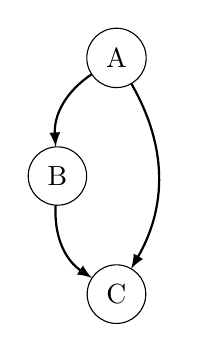
\begin{tikzpicture}[scale=1.0, >=latex, inner sep=0pt, outer sep=0pt, label distance=2pt]
%\draw[step=0.25cm,style=help lines, line width=0.1pt] (-2.5,-3) grid (2.5,3);
%\draw[step=1cm,style=help lines, line width=0.8pt] (-2.5,-3) grid (2.5,3);
%-----
\node[draw, circle, inner sep=4pt] (A) at (0,1.5) {A};
\node[draw, circle, inner sep=4pt] (B) at (-0.75,0) {B};
\node[draw, circle, inner sep=4pt] (C) at (0,-1.5) {C};
\draw[bend right, ->, line width=0.8pt] (A) to (B);
\draw[bend left, ->, line width=0.8pt] (A) to (C);
\draw[bend right, ->, line width=0.8pt] (B) to (C);
\end{tikzpicture}%
}

%--- BUG: NO AUTOMATIC DETECTION BUT IT WORKS WITH \sidefigure!!! WHY???
%\begin{marginfigure}
%\begin{tikzpicture}[scale=1.0, >=latex, inner sep=0pt, outer sep=0pt, label distance=2pt]
%%\draw[step=0.25cm,style=help lines, line width=0.1pt] (-2.5,-3) grid (2.5,3);
%%\draw[step=1cm,style=help lines, line width=0.8pt] (-2.5,-3) grid (2.5,3);
%%-----
%\node[draw, circle, inner sep=4pt] (A) at (0,1.5) {A};
%\node[draw, circle, inner sep=4pt] (B) at (-0.75,0) {B};
%\node[draw, circle, inner sep=4pt] (C) at (0,-1.5) {C};
%\draw[bend right, ->, line width=0.8pt] (A) to (B);
%\draw[bend left, ->, line width=0.8pt] (A) to (C);
%\draw[bend right, ->, line width=0.8pt] (B) to (C);
%\end{tikzpicture}
%\caption{\label{fig:VI.1}Graphe orienté.}
%\end{marginfigure}

La question est alors de savoir comment représenter un graphe par une structure de données. Une première manière est d'utiliser un graphe dit d’adjacence qui, au moyen d'un booléen va dire si deux nœuds sont en relation ou non. Une autre façon de faire est de passer par une liste qui va répertorier les nœuds voisins.

\subsubsection[Parcours de graphe]{Parcours de graphe}
\label{subsub:VI.1.2.2}

La \cref{fig:VI.2} illustre le graphe de la présente partie \qnameref{part:II}. Les différents liens (les arêtes fléchées) indiquent les dépendances entre les séquences.

\vspace{4pt}
\begin{jazzfigure}
\Centering
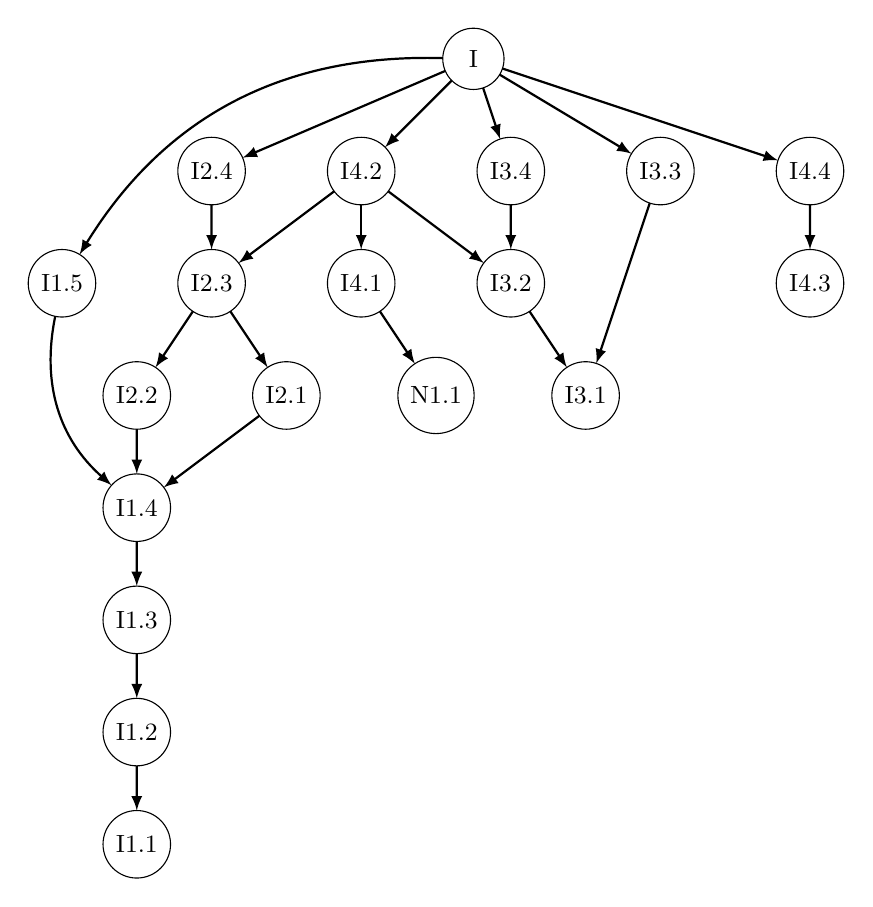
\begin{tikzpicture}[scale=0.95, >=latex, inner sep=0pt, outer sep=0pt, label distance=2pt, font=\small]
%\draw[step=0.25cm,style=help lines, line width=0.1pt] (-5,-3) grid (5,3);
%\draw[step=1cm,style=help lines, line width=0.8pt] (-5,-3) grid (5,3);
%-----
\node[draw, circle, inner sep=3pt] (I) at (0,3.5) {\phantom{3}I\phantom{3}};
\node[draw, circle, inner sep=3pt] (I24) at (-3.5,2.0) {I2.4};
\node[draw, circle, inner sep=3pt] (I42) at (-1.5,2.0) {I4.2};
\node[draw, circle, inner sep=3pt] (I34) at (0.5,2.0) {I3.4};
\node[draw, circle, inner sep=3pt] (I33) at (2.5,2.0) {I3.3};
\node[draw, circle, inner sep=3pt] (I44) at (4.5,2.0) {I4.4};
%---
\node[draw, circle, inner sep=3pt] (I15) at (-5.5,0.5) {I1.5};
\node[draw, circle, inner sep=3pt] (I23) at (-3.5,0.5) {I2.3};
\node[draw, circle, inner sep=3pt] (I41) at (-1.5,0.5) {I4.1};
\node[draw, circle, inner sep=3pt] (I32) at (0.5,0.5) {I3.2};
\node[draw, circle, inner sep=3pt] (I43) at (4.5,0.5) {I4.3};
%---
\node[draw, circle, inner sep=3pt] (I22) at (-4.5,-1) {I2.2};
\node[draw, circle, inner sep=3pt] (I21) at (-2.5,-1) {I2.1};
\node[draw, circle, inner sep=3pt] (N11) at (-0.5,-1) {N1.1};
\node[draw, circle, inner sep=3pt] (I31) at (1.5,-1) {I3.1};
%---
\node[draw, circle, inner sep=3pt] (I14) at (-4.5,-2.5) {I1.4};
\node[draw, circle, inner sep=3pt] (I13) at (-4.5,-4.0) {I1.3};
\node[draw, circle, inner sep=3pt] (I12) at (-4.5,-5.5) {I1.2};
\node[draw, circle, inner sep=3pt] (I11) at (-4.5,-7.0) {I1.1};
%------
\draw[->, line width=0.8pt] (I) to (I24);
\draw[->, line width=0.8pt] (I) to (I42);
\draw[->, line width=0.8pt] (I) to (I34);
\draw[->, line width=0.8pt] (I) to (I33);
\draw[->, line width=0.8pt] (I) to (I44);
%---
\draw[bend right, ->, line width=0.8pt] (I) to (I15);
\draw[->, line width=0.8pt] (I24) to (I23);
\draw[->, line width=0.8pt] (I42) to (I23);
\draw[->, line width=0.8pt] (I42) to (I41);
\draw[->, line width=0.8pt] (I42) to (I32);
\draw[->, line width=0.8pt] (I34) to (I32);
\draw[->, line width=0.8pt] (I33) to (I31);
\draw[->, line width=0.8pt] (I44) to (I43);
%---
\draw[->, line width=0.8pt] (I23) to (I22);
\draw[->, line width=0.8pt] (I23) to (I21);
\draw[->, line width=0.8pt] (I41) to (N11);
\draw[->, line width=0.8pt] (I32) to (I31);
%---
\draw[bend right, ->, line width=0.8pt] (I15) to (I14);
\draw[->, line width=0.8pt] (I22) to (I14);
\draw[->, line width=0.8pt] (I21) to (I14);
%---
\draw[->, line width=0.8pt] (I14) to (I13);
\draw[->, line width=0.8pt] (I13) to (I12);
\draw[->, line width=0.8pt] (I12) to (I11);
\end{tikzpicture}
\caption{\label{fig:VI.2}Graphe des séquences de la partie \qnameref{part:II}.}
\end{jazzfigure}
\vspace{4pt}

Imaginons vouloir suivre une séquence donnée. Pour ce faire, on veut savoir quelles sont les séquences à suivre au préalable. On peut alors dérouler l'algorithme à suivre.

\begin{algorithm}{Parcours de graphe}
// Entrée : - noeud initial n
//          - graphe de dépendance g 
//            sous forme de liste de voisins
// Sortie : - liste des descendants de n (inclus)

res §$\leftarrow$§ vide;
à_traiter §$\leftarrow$§ vide;
à_traiter §$\leftarrow$§ ajouter(n, à_traiter);

TantQue (à_traiter n'est pas vide) Faire
  x §$\leftarrow$§ tête(à_traiter);
  à_traiter §$\leftarrow$§ queue(à_traiter);
  res §$\leftarrow$§ ajouter(x, res);
  l §$\leftarrow$§ g[x]; // Liste des fils de x
  à_traiter §$\leftarrow$§ ajouter(l, à_traiter);
FinTantQue
\end{algorithm}

On montre en \cref{fig:VI.3,fig:VI.4} le déroulé de l'algorithme en partant du nœud « I4.2 ». Les nœuds à traiter sont en rouge, la variable temporaire est en bleu et le résultat en vert.

\vspace*{-4pt}
\begin{jazzfigure*}
\begin{subfigure}{0.49\linewidth}
\Centering
\begin{tikzpicture}[scale=0.725, >=latex, inner sep=0pt, outer sep=0pt, label distance=2pt, font=\scriptsize]
%\draw[step=0.25cm,style=help lines, line width=0.1pt] (-5,-3) grid (5,3);
%\draw[step=1cm,style=help lines, line width=0.8pt] (-5,-3) grid (5,3);
%-----
\node[draw, circle, inner sep=3pt] (I) at (0,3.5) {\phantom{3}I\phantom{3}};
\node[draw, circle, inner sep=3pt] (I24) at (-3.5,2.0) {I2.4};
\node[draw, circle, inner sep=3pt, fill=purered] (I42) at (-1.5,2.0) {\textcolor{black}{I4.2}};
\node[draw, circle, inner sep=3pt] (I34) at (0.5,2.0) {I3.4};
\node[draw, circle, inner sep=3pt] (I33) at (2.5,2.0) {I3.3};
\node[draw, circle, inner sep=3pt] (I44) at (4.5,2.0) {I4.4};
%---
\node[draw, circle, inner sep=3pt] (I15) at (-5.5,0.5) {I1.5};
\node[draw, circle, inner sep=3pt] (I23) at (-3.5,0.5) {I2.3};
\node[draw, circle, inner sep=3pt] (I41) at (-1.5,0.5) {I4.1};
\node[draw, circle, inner sep=3pt] (I32) at (0.5,0.5) {I3.2};
\node[draw, circle, inner sep=3pt] (I43) at (4.5,0.5) {I4.3};
%---
\node[draw, circle, inner sep=3pt] (I22) at (-4.5,-1) {I2.2};
\node[draw, circle, inner sep=3pt] (I21) at (-2.5,-1) {I2.1};
\node[draw, circle, inner sep=3pt] (N11) at (-0.5,-1) {N1.1};
\node[draw, circle, inner sep=3pt] (I31) at (1.5,-1) {I3.1};
%---
\node[draw, circle, inner sep=3pt] (I14) at (-4.5,-2.5) {I1.4};
\node[draw, circle, inner sep=3pt] (I13) at (-4.5,-4.0) {I1.3};
\node[draw, circle, inner sep=3pt] (I12) at (-4.5,-5.5) {I1.2};
\node[draw, circle, inner sep=3pt] (I11) at (-4.5,-7.0) {I1.1};
%------
\draw[->, line width=0.8pt] (I) to (I24);
\draw[->, line width=0.8pt] (I) to (I42);
\draw[->, line width=0.8pt] (I) to (I34);
\draw[->, line width=0.8pt] (I) to (I33);
\draw[->, line width=0.8pt] (I) to (I44);
%---
\draw[bend right, ->, line width=0.8pt] (I) to (I15);
\draw[->, line width=0.8pt] (I24) to (I23);
\draw[->, line width=0.8pt] (I42) to (I23);
\draw[->, line width=0.8pt] (I42) to (I41);
\draw[->, line width=0.8pt] (I42) to (I32);
\draw[->, line width=0.8pt] (I34) to (I32);
\draw[->, line width=0.8pt] (I33) to (I31);
\draw[->, line width=0.8pt] (I44) to (I43);
%---
\draw[->, line width=0.8pt] (I23) to (I22);
\draw[->, line width=0.8pt] (I23) to (I21);
\draw[->, line width=0.8pt] (I41) to (N11);
\draw[->, line width=0.8pt] (I32) to (I31);
%---
\draw[bend right, ->, line width=0.8pt] (I15) to (I14);
\draw[->, line width=0.8pt] (I22) to (I14);
\draw[->, line width=0.8pt] (I21) to (I14);
%---
\draw[->, line width=0.8pt] (I14) to (I13);
\draw[->, line width=0.8pt] (I13) to (I12);
\draw[->, line width=0.8pt] (I12) to (I11);
\end{tikzpicture}
\caption{\label{fig:VI.3a}Initialisation.}
\end{subfigure}\hfill
\begin{subfigure}{0.49\linewidth}
\Centering
\begin{tikzpicture}[scale=0.725, >=latex, inner sep=0pt, outer sep=0pt, label distance=2pt, font=\scriptsize]
%\draw[step=0.25cm,style=help lines, line width=0.1pt] (-5,-3) grid (5,3);
%\draw[step=1cm,style=help lines, line width=0.8pt] (-5,-3) grid (5,3);
%-----
\node[draw, circle, inner sep=3pt] (I) at (0,3.5) {\phantom{3}I\phantom{3}};
\node[draw, circle, inner sep=3pt] (I24) at (-3.5,2.0) {I2.4};
\node[draw, circle, inner sep=3pt, fill=pureblue] (I42) at (-1.5,2.0) {\textcolor{black}{I4.2}};
\node[draw, circle, inner sep=3pt] (I34) at (0.5,2.0) {I3.4};
\node[draw, circle, inner sep=3pt] (I33) at (2.5,2.0) {I3.3};
\node[draw, circle, inner sep=3pt] (I44) at (4.5,2.0) {I4.4};
%---
\node[draw, circle, inner sep=3pt] (I15) at (-5.5,0.5) {I1.5};
\node[draw, circle, inner sep=3pt] (I23) at (-3.5,0.5) {I2.3};
\node[draw, circle, inner sep=3pt] (I41) at (-1.5,0.5) {I4.1};
\node[draw, circle, inner sep=3pt] (I32) at (0.5,0.5) {I3.2};
\node[draw, circle, inner sep=3pt] (I43) at (4.5,0.5) {I4.3};
%---
\node[draw, circle, inner sep=3pt] (I22) at (-4.5,-1) {I2.2};
\node[draw, circle, inner sep=3pt] (I21) at (-2.5,-1) {I2.1};
\node[draw, circle, inner sep=3pt] (N11) at (-0.5,-1) {N1.1};
\node[draw, circle, inner sep=3pt] (I31) at (1.5,-1) {I3.1};
%---
\node[draw, circle, inner sep=3pt] (I14) at (-4.5,-2.5) {I1.4};
\node[draw, circle, inner sep=3pt] (I13) at (-4.5,-4.0) {I1.3};
\node[draw, circle, inner sep=3pt] (I12) at (-4.5,-5.5) {I1.2};
\node[draw, circle, inner sep=3pt] (I11) at (-4.5,-7.0) {I1.1};
%------
\draw[->, line width=0.8pt] (I) to (I24);
\draw[->, line width=0.8pt] (I) to (I42);
\draw[->, line width=0.8pt] (I) to (I34);
\draw[->, line width=0.8pt] (I) to (I33);
\draw[->, line width=0.8pt] (I) to (I44);
%---
\draw[bend right, ->, line width=0.8pt] (I) to (I15);
\draw[->, line width=0.8pt] (I24) to (I23);
\draw[->, line width=0.8pt] (I42) to (I23);
\draw[->, line width=0.8pt] (I42) to (I41);
\draw[->, line width=0.8pt] (I42) to (I32);
\draw[->, line width=0.8pt] (I34) to (I32);
\draw[->, line width=0.8pt] (I33) to (I31);
\draw[->, line width=0.8pt] (I44) to (I43);
%---
\draw[->, line width=0.8pt] (I23) to (I22);
\draw[->, line width=0.8pt] (I23) to (I21);
\draw[->, line width=0.8pt] (I41) to (N11);
\draw[->, line width=0.8pt] (I32) to (I31);
%---
\draw[bend right, ->, line width=0.8pt] (I15) to (I14);
\draw[->, line width=0.8pt] (I22) to (I14);
\draw[->, line width=0.8pt] (I21) to (I14);
%---
\draw[->, line width=0.8pt] (I14) to (I13);
\draw[->, line width=0.8pt] (I13) to (I12);
\draw[->, line width=0.8pt] (I12) to (I11);
\end{tikzpicture}
\caption{\label{fig:VI.3b}Traitement de « I4.2 ».}
\end{subfigure}\\[4pt]
\begin{subfigure}{0.49\linewidth}
\Centering
\begin{tikzpicture}[scale=0.725, >=latex, inner sep=0pt, outer sep=0pt, label distance=2pt, font=\scriptsize]
%\draw[step=0.25cm,style=help lines, line width=0.1pt] (-5,-3) grid (5,3);
%\draw[step=1cm,style=help lines, line width=0.8pt] (-5,-3) grid (5,3);
%-----
\node[draw, circle, inner sep=3pt] (I) at (0,3.5) {\phantom{3}I\phantom{3}};
\node[draw, circle, inner sep=3pt] (I24) at (-3.5,2.0) {I2.4};
\node[draw, circle, inner sep=3pt, fill=puregreen] (I42) at (-1.5,2.0) {\textcolor{black}{I4.2}};
\node[draw, circle, inner sep=3pt] (I34) at (0.5,2.0) {I3.4};
\node[draw, circle, inner sep=3pt] (I33) at (2.5,2.0) {I3.3};
\node[draw, circle, inner sep=3pt] (I44) at (4.5,2.0) {I4.4};
%---
\node[draw, circle, inner sep=3pt] (I15) at (-5.5,0.5) {I1.5};
\node[draw, circle, inner sep=3pt, fill=purered] (I23) at (-3.5,0.5) {I2.3};
\node[draw, circle, inner sep=3pt, fill=purered] (I41) at (-1.5,0.5) {I4.1};
\node[draw, circle, inner sep=3pt, fill=purered] (I32) at (0.5,0.5) {I3.2};
\node[draw, circle, inner sep=3pt] (I43) at (4.5,0.5) {I4.3};
%---
\node[draw, circle, inner sep=3pt] (I22) at (-4.5,-1) {I2.2};
\node[draw, circle, inner sep=3pt] (I21) at (-2.5,-1) {I2.1};
\node[draw, circle, inner sep=3pt] (N11) at (-0.5,-1) {N1.1};
\node[draw, circle, inner sep=3pt] (I31) at (1.5,-1) {I3.1};
%---
\node[draw, circle, inner sep=3pt] (I14) at (-4.5,-2.5) {I1.4};
\node[draw, circle, inner sep=3pt] (I13) at (-4.5,-4.0) {I1.3};
\node[draw, circle, inner sep=3pt] (I12) at (-4.5,-5.5) {I1.2};
\node[draw, circle, inner sep=3pt] (I11) at (-4.5,-7.0) {I1.1};
%------
\draw[->, line width=0.8pt] (I) to (I24);
\draw[->, line width=0.8pt] (I) to (I42);
\draw[->, line width=0.8pt] (I) to (I34);
\draw[->, line width=0.8pt] (I) to (I33);
\draw[->, line width=0.8pt] (I) to (I44);
%---
\draw[bend right, ->, line width=0.8pt] (I) to (I15);
\draw[->, line width=0.8pt] (I24) to (I23);
\draw[->, line width=0.8pt] (I42) to (I23);
\draw[->, line width=0.8pt] (I42) to (I41);
\draw[->, line width=0.8pt] (I42) to (I32);
\draw[->, line width=0.8pt] (I34) to (I32);
\draw[->, line width=0.8pt] (I33) to (I31);
\draw[->, line width=0.8pt] (I44) to (I43);
%---
\draw[->, line width=0.8pt] (I23) to (I22);
\draw[->, line width=0.8pt] (I23) to (I21);
\draw[->, line width=0.8pt] (I41) to (N11);
\draw[->, line width=0.8pt] (I32) to (I31);
%---
\draw[bend right, ->, line width=0.8pt] (I15) to (I14);
\draw[->, line width=0.8pt] (I22) to (I14);
\draw[->, line width=0.8pt] (I21) to (I14);
%---
\draw[->, line width=0.8pt] (I14) to (I13);
\draw[->, line width=0.8pt] (I13) to (I12);
\draw[->, line width=0.8pt] (I12) to (I11);
\end{tikzpicture}
\caption{\label{fig:VI.3c}Résultat de « I4.2 » avec trois fils à traiter.}
\end{subfigure}\hfill
\begin{subfigure}{0.49\linewidth}
\Centering
\begin{tikzpicture}[scale=0.725, >=latex, inner sep=0pt, outer sep=0pt, label distance=2pt, font=\scriptsize]
%\draw[step=0.25cm,style=help lines, line width=0.1pt] (-5,-3) grid (5,3);
%\draw[step=1cm,style=help lines, line width=0.8pt] (-5,-3) grid (5,3);
%-----
\node[draw, circle, inner sep=3pt] (I) at (0,3.5) {\phantom{3}I\phantom{3}};
\node[draw, circle, inner sep=3pt] (I24) at (-3.5,2.0) {I2.4};
\node[draw, circle, inner sep=3pt, fill=puregreen] (I42) at (-1.5,2.0) {\textcolor{black}{I4.2}};
\node[draw, circle, inner sep=3pt] (I34) at (0.5,2.0) {I3.4};
\node[draw, circle, inner sep=3pt] (I33) at (2.5,2.0) {I3.3};
\node[draw, circle, inner sep=3pt] (I44) at (4.5,2.0) {I4.4};
%---
\node[draw, circle, inner sep=3pt] (I15) at (-5.5,0.5) {I1.5};
\node[draw, circle, inner sep=3pt, fill=purered] (I23) at (-3.5,0.5) {I2.3};
\node[draw, circle, inner sep=3pt, fill=purered] (I41) at (-1.5,0.5) {I4.1};
\node[draw, circle, inner sep=3pt, fill=pureblue] (I32) at (0.5,0.5) {I3.2};
\node[draw, circle, inner sep=3pt] (I43) at (4.5,0.5) {I4.3};
%---
\node[draw, circle, inner sep=3pt] (I22) at (-4.5,-1) {I2.2};
\node[draw, circle, inner sep=3pt] (I21) at (-2.5,-1) {I2.1};
\node[draw, circle, inner sep=3pt] (N11) at (-0.5,-1) {N1.1};
\node[draw, circle, inner sep=3pt] (I31) at (1.5,-1) {I3.1};
%---
\node[draw, circle, inner sep=3pt] (I14) at (-4.5,-2.5) {I1.4};
\node[draw, circle, inner sep=3pt] (I13) at (-4.5,-4.0) {I1.3};
\node[draw, circle, inner sep=3pt] (I12) at (-4.5,-5.5) {I1.2};
\node[draw, circle, inner sep=3pt] (I11) at (-4.5,-7.0) {I1.1};
%------
\draw[->, line width=0.8pt] (I) to (I24);
\draw[->, line width=0.8pt] (I) to (I42);
\draw[->, line width=0.8pt] (I) to (I34);
\draw[->, line width=0.8pt] (I) to (I33);
\draw[->, line width=0.8pt] (I) to (I44);
%---
\draw[bend right, ->, line width=0.8pt] (I) to (I15);
\draw[->, line width=0.8pt] (I24) to (I23);
\draw[->, line width=0.8pt] (I42) to (I23);
\draw[->, line width=0.8pt] (I42) to (I41);
\draw[->, line width=0.8pt] (I42) to (I32);
\draw[->, line width=0.8pt] (I34) to (I32);
\draw[->, line width=0.8pt] (I33) to (I31);
\draw[->, line width=0.8pt] (I44) to (I43);
%---
\draw[->, line width=0.8pt] (I23) to (I22);
\draw[->, line width=0.8pt] (I23) to (I21);
\draw[->, line width=0.8pt] (I41) to (N11);
\draw[->, line width=0.8pt] (I32) to (I31);
%---
\draw[bend right, ->, line width=0.8pt] (I15) to (I14);
\draw[->, line width=0.8pt] (I22) to (I14);
\draw[->, line width=0.8pt] (I21) to (I14);
%---
\draw[->, line width=0.8pt] (I14) to (I13);
\draw[->, line width=0.8pt] (I13) to (I12);
\draw[->, line width=0.8pt] (I12) to (I11);
\end{tikzpicture}
\caption{\label{fig:VI.3d}Résultat une fois toutes les branches de « I4.2 » traitées.}
\end{subfigure}
\caption{\label{fig:VI.3}Parcours de graphe : déroulé de l'algorithme.}
\vspace*{-4pt}
\end{jazzfigure*}

Partant de « I4.2 », on commence par le traiter, donc ce nœud passe en bleu, puis on s'attache à traiter tous ses fils. Le nœud « I4.2 » passe en vert et on doit traiter successivement les trois nœuds en rouge. Imaginons que le premier fils à traiter soit « I3.2 », il passe en bleu, puis en vert une fois le traitement effectué. Il reste dans cette branche à traiter le seul  fils de « I3.2 ». Au final, pour suivre la séquence « I4.2 », il faut d'abord suivre l'arborescence des séquences donnée en \cref{fig:VI.4b}.


\begin{jazzfigure*}
\begin{subfigure}{0.49\linewidth}
\Centering
\begin{tikzpicture}[scale=0.725, >=latex, inner sep=0pt, outer sep=0pt, label distance=2pt, font=\scriptsize]
%\draw[step=0.25cm,style=help lines, line width=0.1pt] (-5,-3) grid (5,3);
%\draw[step=1cm,style=help lines, line width=0.8pt] (-5,-3) grid (5,3);
%-----
\node[draw, circle, inner sep=3pt] (I) at (0,3.5) {\phantom{3}I\phantom{3}};
\node[draw, circle, inner sep=3pt] (I24) at (-3.5,2.0) {I2.4};
\node[draw, circle, inner sep=3pt, fill=puregreen] (I42) at (-1.5,2.0) {\textcolor{black}{I4.2}};
\node[draw, circle, inner sep=3pt] (I34) at (0.5,2.0) {I3.4};
\node[draw, circle, inner sep=3pt] (I33) at (2.5,2.0) {I3.3};
\node[draw, circle, inner sep=3pt] (I44) at (4.5,2.0) {I4.4};
%---
\node[draw, circle, inner sep=3pt] (I15) at (-5.5,0.5) {I1.5};
\node[draw, circle, inner sep=3pt, fill=purered] (I23) at (-3.5,0.5) {I2.3};
\node[draw, circle, inner sep=3pt, fill=purered] (I41) at (-1.5,0.5) {I4.1};
\node[draw, circle, inner sep=3pt, fill=puregreen] (I32) at (0.5,0.5) {I3.2};
\node[draw, circle, inner sep=3pt] (I43) at (4.5,0.5) {I4.3};
%---
\node[draw, circle, inner sep=3pt] (I22) at (-4.5,-1) {I2.2};
\node[draw, circle, inner sep=3pt] (I21) at (-2.5,-1) {I2.1};
\node[draw, circle, inner sep=3pt] (N11) at (-0.5,-1) {N1.1};
\node[draw, circle, inner sep=3pt, fill=purered] (I31) at (1.5,-1) {I3.1};
%---
\node[draw, circle, inner sep=3pt] (I14) at (-4.5,-2.5) {I1.4};
\node[draw, circle, inner sep=3pt] (I13) at (-4.5,-4.0) {I1.3};
\node[draw, circle, inner sep=3pt] (I12) at (-4.5,-5.5) {I1.2};
\node[draw, circle, inner sep=3pt] (I11) at (-4.5,-7.0) {I1.1};
%------
\draw[->, line width=0.8pt] (I) to (I24);
\draw[->, line width=0.8pt] (I) to (I42);
\draw[->, line width=0.8pt] (I) to (I34);
\draw[->, line width=0.8pt] (I) to (I33);
\draw[->, line width=0.8pt] (I) to (I44);
%---
\draw[bend right, ->, line width=0.8pt] (I) to (I15);
\draw[->, line width=0.8pt] (I24) to (I23);
\draw[->, line width=0.8pt] (I42) to (I23);
\draw[->, line width=0.8pt] (I42) to (I41);
\draw[->, line width=0.8pt] (I42) to (I32);
\draw[->, line width=0.8pt] (I34) to (I32);
\draw[->, line width=0.8pt] (I33) to (I31);
\draw[->, line width=0.8pt] (I44) to (I43);
%---
\draw[->, line width=0.8pt] (I23) to (I22);
\draw[->, line width=0.8pt] (I23) to (I21);
\draw[->, line width=0.8pt] (I41) to (N11);
\draw[->, line width=0.8pt] (I32) to (I31);
%---
\draw[bend right, ->, line width=0.8pt] (I15) to (I14);
\draw[->, line width=0.8pt] (I22) to (I14);
\draw[->, line width=0.8pt] (I21) to (I14);
%---
\draw[->, line width=0.8pt] (I14) to (I13);
\draw[->, line width=0.8pt] (I13) to (I12);
\draw[->, line width=0.8pt] (I12) to (I11);
\end{tikzpicture}
\caption{\label{fig:VI.4a}Résultat de « I3.2 » avec un fils à traiter.}
\end{subfigure}\hfill
\begin{subfigure}{0.49\linewidth}
\Centering
\begin{tikzpicture}[scale=0.725, >=latex, inner sep=0pt, outer sep=0pt, label distance=2pt, font=\scriptsize]
%\draw[step=0.25cm,style=help lines, line width=0.1pt] (-5,-3) grid (5,3);
%\draw[step=1cm,style=help lines, line width=0.8pt] (-5,-3) grid (5,3);
%-----
\node[draw, circle, inner sep=3pt] (I) at (0,3.5) {\phantom{3}I\phantom{3}};
\node[draw, circle, inner sep=3pt] (I24) at (-3.5,2.0) {I2.4};
\node[draw, circle, inner sep=3pt, fill=puregreen] (I42) at (-1.5,2.0) {\textcolor{black}{I4.2}};
\node[draw, circle, inner sep=3pt] (I34) at (0.5,2.0) {I3.4};
\node[draw, circle, inner sep=3pt] (I33) at (2.5,2.0) {I3.3};
\node[draw, circle, inner sep=3pt] (I44) at (4.5,2.0) {I4.4};
%---
\node[draw, circle, inner sep=3pt] (I15) at (-5.5,0.5) {I1.5};
\node[draw, circle, inner sep=3pt, fill=puregreen] (I23) at (-3.5,0.5) {I2.3};
\node[draw, circle, inner sep=3pt, fill=puregreen] (I41) at (-1.5,0.5) {I4.1};
\node[draw, circle, inner sep=3pt, fill=puregreen] (I32) at (0.5,0.5) {I3.2};
\node[draw, circle, inner sep=3pt] (I43) at (4.5,0.5) {I4.3};
%---
\node[draw, circle, inner sep=3pt, fill=puregreen] (I22) at (-4.5,-1) {I2.2};
\node[draw, circle, inner sep=3pt, fill=puregreen] (I21) at (-2.5,-1) {I2.1};
\node[draw, circle, inner sep=3pt, fill=puregreen] (N11) at (-0.5,-1) {N1.1};
\node[draw, circle, inner sep=3pt, fill=puregreen] (I31) at (1.5,-1) {I3.1};
%---
\node[draw, circle, inner sep=3pt, fill=puregreen] (I14) at (-4.5,-2.5) {I1.4};
\node[draw, circle, inner sep=3pt, fill=puregreen] (I13) at (-4.5,-4.0) {I1.3};
\node[draw, circle, inner sep=3pt, fill=puregreen] (I12) at (-4.5,-5.5) {I1.2};
\node[draw, circle, inner sep=3pt, fill=puregreen] (I11) at (-4.5,-7.0) {I1.1};
%------
\draw[->, line width=0.8pt] (I) to (I24);
\draw[->, line width=0.8pt] (I) to (I42);
\draw[->, line width=0.8pt] (I) to (I34);
\draw[->, line width=0.8pt] (I) to (I33);
\draw[->, line width=0.8pt] (I) to (I44);
%---
\draw[bend right, ->, line width=0.8pt] (I) to (I15);
\draw[->, line width=0.8pt] (I24) to (I23);
\draw[->, line width=0.8pt] (I42) to (I23);
\draw[->, line width=0.8pt] (I42) to (I41);
\draw[->, line width=0.8pt] (I42) to (I32);
\draw[->, line width=0.8pt] (I34) to (I32);
\draw[->, line width=0.8pt] (I33) to (I31);
\draw[->, line width=0.8pt] (I44) to (I43);
%---
\draw[->, line width=0.8pt] (I23) to (I22);
\draw[->, line width=0.8pt] (I23) to (I21);
\draw[->, line width=0.8pt] (I41) to (N11);
\draw[->, line width=0.8pt] (I32) to (I31);
%---
\draw[bend right, ->, line width=0.8pt] (I15) to (I14);
\draw[->, line width=0.8pt] (I22) to (I14);
\draw[->, line width=0.8pt] (I21) to (I14);
%---
\draw[->, line width=0.8pt] (I14) to (I13);
\draw[->, line width=0.8pt] (I13) to (I12);
\draw[->, line width=0.8pt] (I12) to (I11);
\end{tikzpicture}
\caption{\label{fig:VI.4b}Résultat final.}
\end{subfigure}
\caption{\label{fig:VI.4}Parcours de graphe : déroulé de l'algorithme (suite) et résultat final.}
\end{jazzfigure*}

\vspace{-8pt}

\begin{gofurther}
\lightbf{Formation complémentaire}
\begin{itemize}\jazzitem
	\item Partie 4 du \href{https://pixees.fr/classcode/formations/module1/\#partie4}{\#1 Module fondamental : découvrir la programmation créative}, \textsc{Class´Code}. Cette formation pour enseignants du secondaire offre des vidéos accessibles en cliquant sur le pictogramme \faIcon[regular]{play-circle}.
\end{itemize}

\lightbf{Articles}
\begin{itemize}\jazzitem
\item \href{https://interstices.info/les-ingredients-des-algorithmes/}{Les ingrédients des algorithmes}, Gilles \textsc{Dowek}, Thierry \textsc{Viéville}, Jean-Pierre, \textsc{Archambault} , Emmanuel \textsc{Baccelli} et Benjamin \textsc{Wack}, \textsc{Interstices}, 21 avril 2010.
\item \href{https://interstices.info/quest-ce-quun-algorithme/}{Qu’est-ce qu’un algorithme ?}, Philippe \textsc{Flajolet} et Étienne \textsc{Parizot}, \textsc{Interstices}, 24 février 2004 ;
%\item \href{https://www.lemonde.fr/blog/binaire/category/si-jetais-un-algorithme/}{Petit algo deviendra grand}, Jean %\textsc{Vuillemin}, \textsc{Binaire}, 30 janvier 2017 ;
\end{itemize}

\lightbf{Podcast et vidéo}
\begin{itemize}\jazzitem
\item \href{https://interstices.info/a-propos-des-algorithmes/}{À propos des algorithmes}, Marie-Christine \textsc{Rousset}, Intersti\-ces, 15 juillet 2013.
\end{itemize}

\lightbf{Ouvrages}
\begin{itemize}\jazzitem
\item \textit{Apprendre à programmer avec Ocaml : Algorithmes, structures de données}, Sylvain \textsc{Conchon} et Jean-Christophe \textsc{Filliâtre}, \textsc{Eyrolles}, 2014 ;
\item \textit{Programmation efficace --- 128 algorithmes qu’il faut avoir compris et codés en \textsc{Python} au cours de sa vie}, Christoph \textsc{Dürr} et Jill-Jênn \textsc{Vie}, \textsc{Ellipses}, 2016 ;
\item \textit{Algorithms}, Robert \textsc{Sedgewick} et Kevin \textsc{Wayne}, 4\frup{e} éd., \textsc{Addison-Wesley Professional}, 2011 ;
\item \textit{The Art of Computer Programming}, Donald E. \textsc{Knuth}, \textsc{Addison Wesley}, 2011.
\end{itemize}
\end{gofurther}


%----------
\section[Programmation]{Programmation}
\label{sec:VI.2}

Après avoir établi une solution algorithmique d'une problématique, vient le temps de son implémentation effective en tant que programme informatique. Pour cela, il faut pouvoir discuter sereinement avec la machine pour lui indiquer les consignes à respecter. 



\subsection[Langages de programmation]{Langages de programmation}
\label{sub:VI.2.1}

Comment le dialogue ou plutôt les ordres et impératifs se communi\-quent-ils à l'ordinateur ? Ce codage peut désormais se réaliser à l'aide d'une mosaïque de langages différents, mais alors lequel choisir ?

\subsubsection[Langage machine]{Langage machine}
\label{subsub:VI.2.1.1}

\begin{marginvideo}
	[\label{vid:VI.5}Langage machine.]%
	\movie[width=\marginparwidth,showcontrols]%
		{
\includegraphics[width=\marginparwidth]{./Images/Pictograms/film-strip-dark-electric-blue.png}}%
		{./Videos/Chapter06/vidVI-05-machine-language-HD.mp4}%
	\launchvideo{./Videos/Chapter06/vidVI-05-machine-language-HD.mp4}
\end{marginvideo}

\href{https://www.college-de-france.fr/site/gerard-berry/#course}{Gérard \textsc{Berry}} l'a exprimé dans \href{http://rue89.nouvelobs.com/2016/08/26/gerard-berry-lordinateur-est-completement-con-257428}{une interview à Rue89} : « l'ordinateur est complètement con ». Que signifie ce constat fondateur et cette formulation ravageuse, mais claire comme de l'eau de roche ? Cela induit juste que l'ordinateur ne réalise que ce qu'on lui ordonne de faire pas plus, pas moins ; il faut \textit{tout} lui dire, il n'a aucune initiative propre. Il ne sait pas faire quelque chose d'intelligent. La seule intelligence est dans l'esprit du programmeur. 

Le langage machine, comme son nom l'indique, est celui que le processeur comprend. Pour chaque type de processeur un dialecte a été développé pour prendre en compte les particularités propres aux différents processeurs, mais la base est commune.

En fait, l'ordinateur, le \textit{smartphone} ou la tablette ne sont pas des objets magiques. L'algorithme doit leur être prémâché dans ses plus infimes détails. Ce sont des dispositifs électroniques très avancés mais très simples dans leurs fonctionnalités. Leur avantage et leurs performances sont liés à leur rapidité d'exécution des tâches. Il ne savent obéir qu'à des ordres élémentaires qui correspondent aux instructions du langage machine, que l'on nomme également de l'\textit{assembleur}.

Typiquement, le nombre d'instructions possibles est fini et relativement faible. Un processeur sait déplacer des éléments de la mémoire globale à la mémoire locale --- dite vive ou dans les registres ---, comparer deux valeurs ou les ajouter, multiplier, diviser. Il est aussi capable de sauter à un autre point du programme pour réaliser des boucles ou des tests. Un processeur est donc à même de faire des choses très simples et très unitaires.

\vspace{6pt}

\begin{lstlisting}[style=lstassemblerstyle]
      movl    $0, -8(%rbp)
      movl    $7, -4(%rbp)
      cmpl    $0, -4(%rbp)
      jle     .L2
      movl    -4(%rbp), %eax
      addl    %eax, -8(%rbp)
.L2:
      movl    -8(%rbp), %eax 
\end{lstlisting}

\vspace{6pt}

À titre d'illustration, le bout de code ci-dessus est en assembleur X86. L'instruction \texttt{movl} sert à mettre des valeurs dans des registres. Ici, on met la valeur \texttt{0} dans un certain registre, puis la valeur \texttt{7} dans un autre registre. Ensuite, on effectue une comparaison --- instruction \texttt{cmpl} --- entre la valeur \texttt{0} et le contenu du registre numéro \texttt{4}. Puis, à partir de cette comparaison, on fait un test et, en fonction du résultat, on va sauter à un autre point du programme qui est nommé \texttt{.L2}. Dans les deux cas de figure du test, on poursuit différemment les traitements. 

On constate d'emblée que le langage machine est abscons, peu naturel et pas beau... Il est relativement difficile de comprendre la signification du code. Donc la seule conclusion à tirer est qu'on n'a pas du tout envie d'écrire du langage assembleur, c'est pourquoi on va utiliser des langages de plus haut niveau et de la compilation. 

\begin{gofurther}
\lightbf{Articles}
\begin{itemize}\jazzitem
\item \href{https://www.nouvelobs.com/rue89/rue89-le-grand-entretien/20160826.RUE7684/gerard-berry-l-ordinateur-est-completement-con.html}{Gérard \textsc{Berry}. L'ordinateur est complètement con}, Xavier \textsc{La Porte}, \textsc{L'obs avec Rue 89}, 21 novembre 2016.
\item Le \href{https://fr.wikipedia.org/wiki/Assembleur}{langage assembleur}, \textsc{Wikipédia}.
\end{itemize}

\vspace{2pt}
\lightbf{Vidéo}
\begin{itemize}\jazzitem
\item \href{https://videotheque.cnrs.fr/visio=4419}{Gérard Berry : l'homme qui orchestre les ordinateurs}, \textsc{Cnrs}, 2014 (6mn).
\end{itemize}
\end{gofurther}

\vspace{6pt}


\subsubsection[Langage de haut niveau et compilation]{Langage de haut niveau et compilation}
\label{subsub:VI.2.1.2}

\begin{marginvideo}
	[\label{vid:VI.6}Langages et compilation.]%
	\movie[width=\marginparwidth,showcontrols]%
		{
\includegraphics[width=\marginparwidth]{./Images/Pictograms/film-strip-dark-electric-blue.png}}%
		{./Videos/Chapter06/vidVI-06-highlevel-language-HD.mp4}%
	\launchvideo{./Videos/Chapter06/vidVI-06-highlevel-language-HD.mp4}
\end{marginvideo}

Quand on veut écrire un programme, on part d'une idée. Que veut-on faire et calculer ? Après, on pense aux grandes 
lignes, c'est-à-dire à la mise en place d'une espèce de séquençage, comme précisé dans la partie algorithmique. On définit alors l'algorithme et on décide des structures de données. Ensuite, on choisit un langage de programmation en fonction d'un certain nombre de critères --- ce choix est abordé en section suivante --- et on se lance dans l'écriture du code. 

On parle de langage de haut niveau car la sémantique et la syntaxe de ce type de langage se veulent proches de la compréhension de l'humain et non plus de la machine comme avec l'assembleur. Néanmoins, pour que le code que l'on écrit soit compréhensible par l'ordinateur, il faut le traduire en langage machine. C'est là qu'intervient la phase de compilation : obtenir un programme dit \emph{exécutable} et donc exploitable à partir d'un fichier texte constitué d'un ensemble d'instructions correspondant au langage de programmation choisi.

Le compilateur est un programme comme les autres qui agit comme traducteur en prenant en entrée un fichier texte écrit par exemple en C, C++ ou \textsc{Java} et livre un exécutable. Au passage, le compilateur vérifie un certain nombre de règles d'écriture comme la syntaxe ou le typage des variables, mais aussi propose des aides pour la détection des erreurs, voire dispose d'options pour optimiser le programme.

Il existe un second type de langage de haut niveau, les langages dits \emph{interprétés}. Le code source --- au format texte --- n'est plus directement présenté au compilateur, mais confié à ce que l'on appelle un \emph{interpréteur}, qui lui se charge de traduire les instructions en langage machine. Par exemple, \textsc{Perl} ou \textsc{Python} sont des langages interprétés. Ici, c'est l'interpréteur qui a été compilé au préalable en fonction du processeur et du système d'exploitation.

Puisqu'il y a un intermédiaire, les langages interprétés sont généralement plus lents, mais de nos jours ce n'est plus un souci car d'une part, la puissance des machines apporte la transparence et, d'autre part, on peut combiner les langages entre eux sous forme de bibliothèques en fonction des tâches à accomplir. C'est à ce propos la grande force de \textsc{Python}.

Le grand avantage des langages interprétés est, outre l’absence de compilation, d'être multiplate-forme, à savoir qu'un même fichier sour\-ce « tournera » de manière identique quel que soit le système d'exploitation. En quelque sorte, ils sont « encore plus » de haut niveau. À ce titre, \textsc{Python} est exemplaire car, comparativement, se trouve le plus proche du langage naturel.

\begin{gofurther}
\lightbf{Formation complémentaire}
\begin{itemize}\jazzitem
\item \href{https://pixees.fr/classcode/formations/module1/}{\#1 Module fondamental : découvrir la programmation créative}, \textsc{Class´Code}, Partie 1, pour s'initier à la programmation avec \textsc{Scratch} (cela permet de s'adresser aux futurs élèves formés à \textsc{Scratch} au collège ou en périscolaire).
\item Le \href{https://fr.wikipedia.org/wiki/Assembleur}{langage assembleur}, \textsc{Wikipédia}.
\end{itemize}

\vspace{2pt}
\lightbf{Articles}
\begin{itemize}\jazzitem
\item \href{https://fr.wikipedia.org/wiki/Compilateur}{Compilateur}, \textsc{Wikipédia}.
\item \href{https://fr.wikipedia.org/wiki/Grace_Hopper}{Grace Hopper, conceptrice du premier compilateur}, \textsc{Wikipédia}.
\item \href{https://interstices.info/comment-faire-confiance-a-un-compilateur/}{Comment faire confiance à un compilateur ?} Xavier \textsc{Leroy}, \textsc{Interstices}, 21 mai 2010.
\end{itemize}

\vspace{2pt}
\lightbf{Podcast}
\begin{itemize}\jazzitem
\item \href{https://interstices.info/a-propos-des-compilateurs/}{À propos des compilateurs}, Sandrine \textsc{Blazy} et Joanna \textsc{Jongwane}, \textsc{Interstices}, 29 mars 2012, (09mn, 30s).
\end{itemize}
\end{gofurther}


\subsection[Paradigmes de programmation]{Paradigmes de programmation}
\label{sub:VI.2.2}

\subsubsection[Bogues]{Bogues}
\label{subsub:VI.2.2.1}

\begin{marginvideo}
	[\label{vid:VI.7}Histoire de \textup{bugs}.]%
	\movie[width=\marginparwidth,showcontrols]%
		{
\includegraphics[width=\marginparwidth]{./Images/Pictograms/film-strip-dark-electric-blue.png}}%
		{./Videos/Chapter06/vidVI-07-bugs-HD.mp4}%
	\launchvideo{./Videos/Chapter06/vidVI-07-bugs-HD.mp4}
\end{marginvideo}

Les \textit{bugs} jalonnent l'histoire de l'informatique. Pour le grand public, peut-être que le plus célèbre serait le « \textit{bug} de l'an 2000 ». Il y en a d'autres, parfois dramatique, citons deux exemples.

La première anecdote est liée à l'USS Yorktown, un navire américain de guerre qui a été lancé en 1996 avec un programme \textit{Navy's Smart Ship} qui signifie « bateau intelligent ». Lors d'essais, un membre d'équipage s'est trompé sur ce qu'il rentrait comme valeur d'entrée dans la machine, il a rentré un zéro sur une valeur qui, en théorie, n'était pas censée être nulle. La conséquence, c'est qu'il y a eu dans le programme une division par zéro qui est remontée et a complètement planté le système d'exploitation. La conséquence est que plus rien ne fonctionnait sur le bateau, pas même les moteurs.

On peut trouver plus amples détails sur \href{https://en.wikipedia.org/wiki/USS_Yorktown_(CG-48)}{\textsc{Wikipédia}} mais, ce qu'il faut retenir, c'est que les valeurs d'entrée doivent être testées parce qu'on n'est jamais sûr que l'utilisateur final est bien conscient qu'il y a des valeurs interdites. Par ailleurs, ce genre de valeur non attendue est également une porte d'entrée pour les attaques sur les programmes. 

\sidegraphic{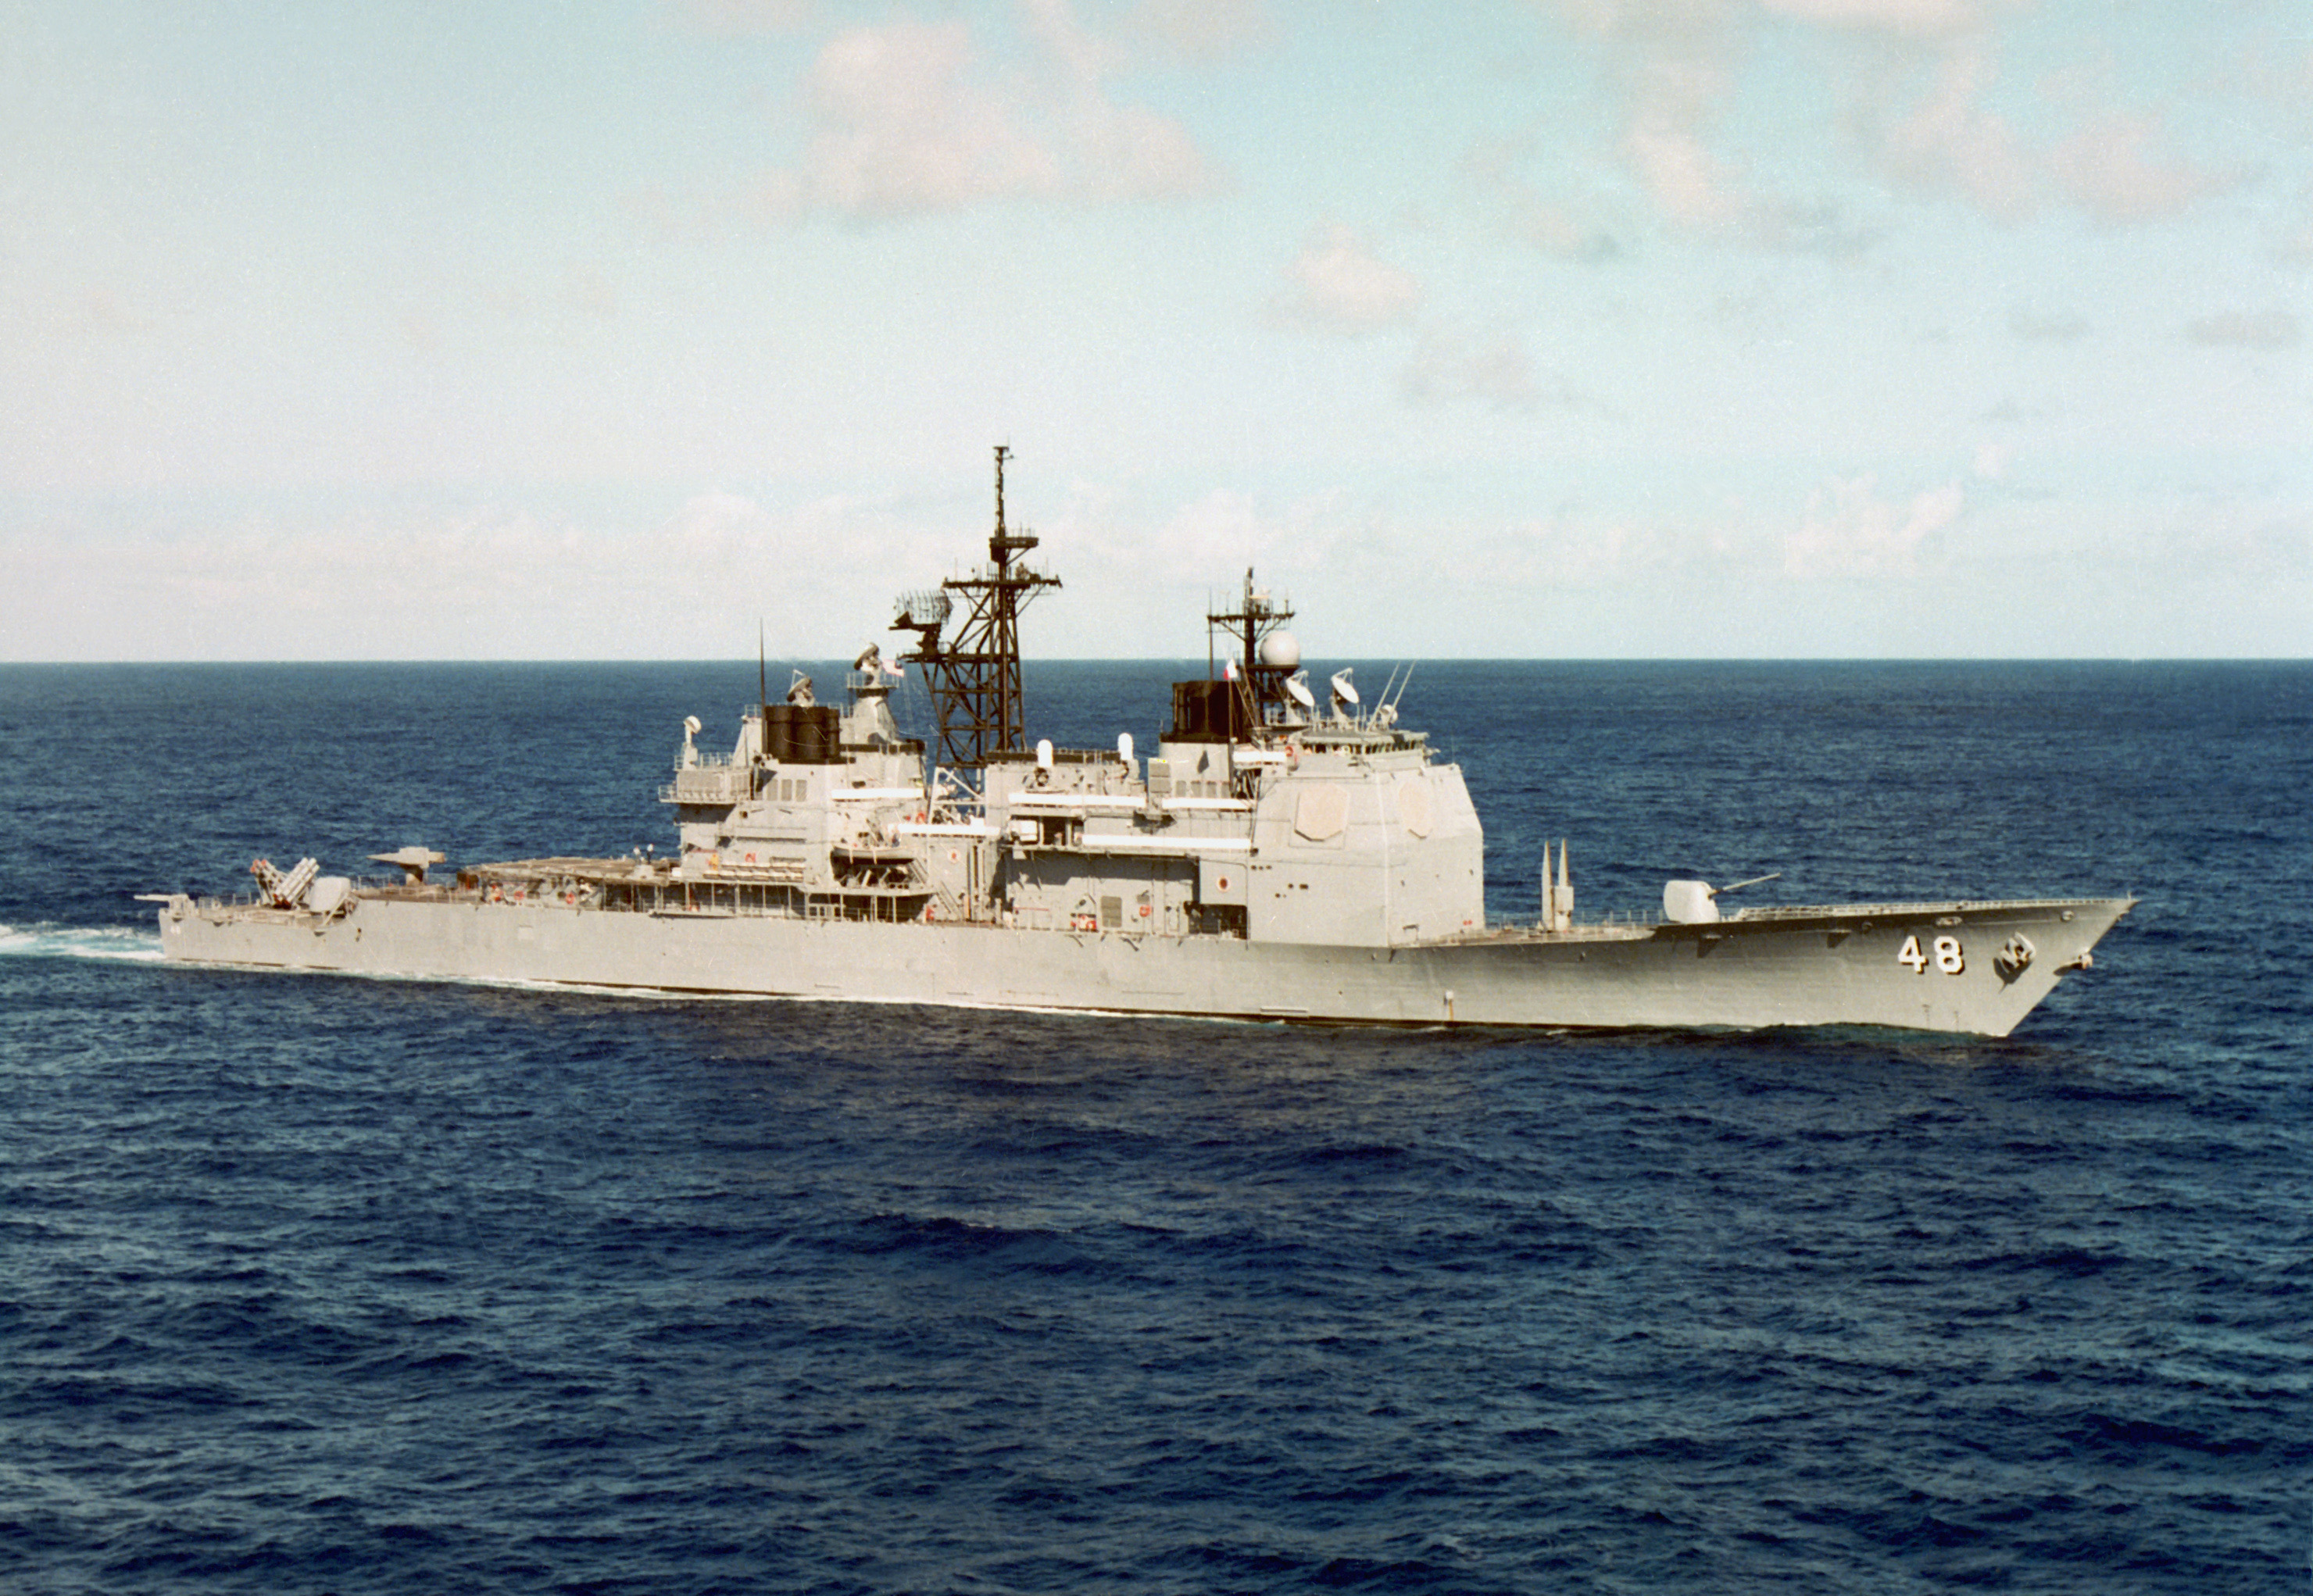
\includegraphics[width=\linewidth]{graphVI-02-uss-yorktown-cg48-circa1985.jpg}}%
Un autre exemple concerne le lanceur de satellites Ariane 5, successeur d'Ariane 4, qui fonctionnait très bien avec un programme spécifique. Lors de la conception d'Arianne 5 ce programme a été repris à la lettre et implémenté sans autre vérification. Il se trouve simplement que le lanceur Arianne 5 est plus lourd que son prédécesseur et des valeurs maximales qui étaient correctes pour Ariane 4 ne l'étaient plus pour Ariane 5.

\href{https://fr.wikipedia.org/wiki/Vol_501_d\%27Ariane_5}{Au premier lancer d'Ariane 5}, les valeurs maximales ont été dépassées et, en informatique, quand on dépasse les valeurs maximales autorisées d'un entier ou d'un flottant, il se passe des choses bizarres, en particulier pour les nombres à virgule flottante, on peut avoir des valeurs très grandes qui deviennent très petites ou des entiers positifs qui virent en négatif. Aussi, une valeur complètement absurde a fait que le lanceur de satellites a commencé à partir sur le côté et il a fallu le détruire pour ne pas qu'il tombe sur les habitations. 

\pagebreak

\sidegraphic{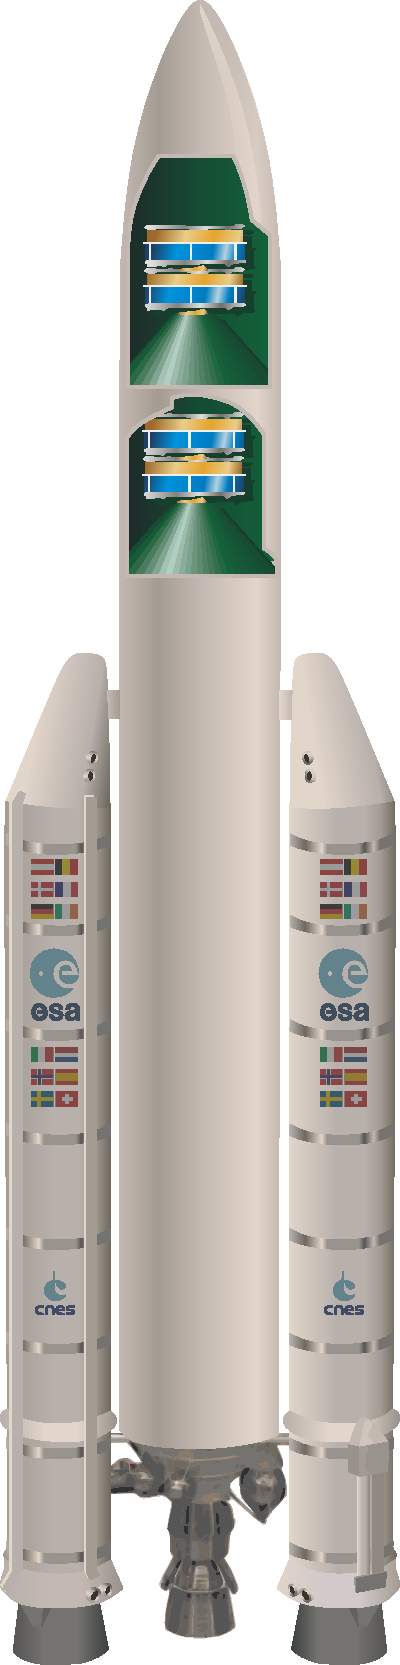
\includegraphics[width=0.4\linewidth]{graphVI-03-ariane-501.pdf}}%
Ici, la conclusion est qu'il faut faire attention aux variables qu'on utilise et à leur type pour être sûr qu'on ne va pas dépasser les valeurs maximales et minimales autorisées (par exemple des tableaux). 

Alors qu'est-ce que c'est qu'un \textit{bug} ? C'est \textit{in fine} le résultat d'un programme que l'utilisateur ne désire pas. Cela peut être une erreur de programmation --- autrement dit qu'effectivement la personne qui a programmé s'est trompée ---, l'oubli d'un cas particulier, une typo ou une coquille, un dépassement de capacités comme dans l'exemple précédent, un accès illicite à la mémoire --- c'est-à-dire accéder à un morceau de mémoire qui n'était pas prévu et donc qui n'était pas initialisé avec une valeur correcte ---, etc.

Il existe aussi une catégorie de bug plus sournois, mais finalement au moins aussi fréquent, relatifs aux erreurs de communication, c'est-à-dire qu'effectivement, entre la personne qui a demandé le programme et la personne qui l'a programmé à la fin, il y a eu une mauvaise compréhension sur les valeurs d'entrée, sur ce que devait faire le programme, ou tout autre état de cause. 
 
Il peut également y avoir une erreur de communication entre deux programmeurs. Les programmes actuels sont en effet écrits par des milliers de personnes qui doivent interagir et comprendre ce que fait le morceau de programme des autres développeurs. La \cref{fig:VI.5} en apporte l'illustration en comparant les nombres de lignes de code pour certaines applications connues. On remarque que déjà un \textit{pacemaker} et ses quelques 100\,000 lignes de code est difficile à programmer par une seule personne, qu'en est-il alors de \textsc{Facebook} et et ses soixante millions de lignes de code ? Il y a fort à parier que des \textit{bugs} se glissent dans les programmes et les fassent planter de temps à autres.


%- See: https://tex.stackexchange.com/questions/141087/how-to-clarify-and-enliven-a-dense-table
%-      https://tex.stackexchange.com/questions/156964/guide-to-draw-charts-basic-pie-bar-from-data
%-      https://tex.stackexchange.com/questions/101320/grouped-bar-chart/
%-      https://tex.stackexchange.com/questions/31525/how-to-minimize-the-ink-to-data-ratio-for-pgfplots

%    Unix v1.0 (1971)            & 0.01  \\
%    Average iPhone app          & 0.04  \\

\pgfplotstableread[row sep=\\,col sep=&]{
    Name                        & Value \\
    Pacemaker                   & 0.08  \\
    Photoshop v1.0 (1990)       & 0.1   \\
    Linux Kernel 2.2.0          & 2     \\
    Hubble Space Telescope      & 2     \\
    Windows 3.1 (1992)          & 2.5   \\
    Photoshop C.S.6             & 4.5   \\
    Windows NT 3.1 (1993)       & 4.5   \\
    Linux Kernel 2.6.0 (2003)   & 5.2   \\
    Google Chrome               & 6.7   \\
    Firefox                     & 9.7   \\
    Android                     & 12    \\
    Boeing 787                  & 14    \\
    Linux 3.1                   & 15    \\
    Apache Open Office          & 23    \\
    Windows 2000 (2001)         & 29    \\
    Windows XP (2001)           & 40    \\
    Microsoft Office 2013       & 45    \\
    Facebook                    & 62    \\
    Debian 5.0 Codebase         & 68    \\
    Mac OS X Tiger v10.4        & 86    \\
    }\lineofcodes

\begin{jazzfigure*}
%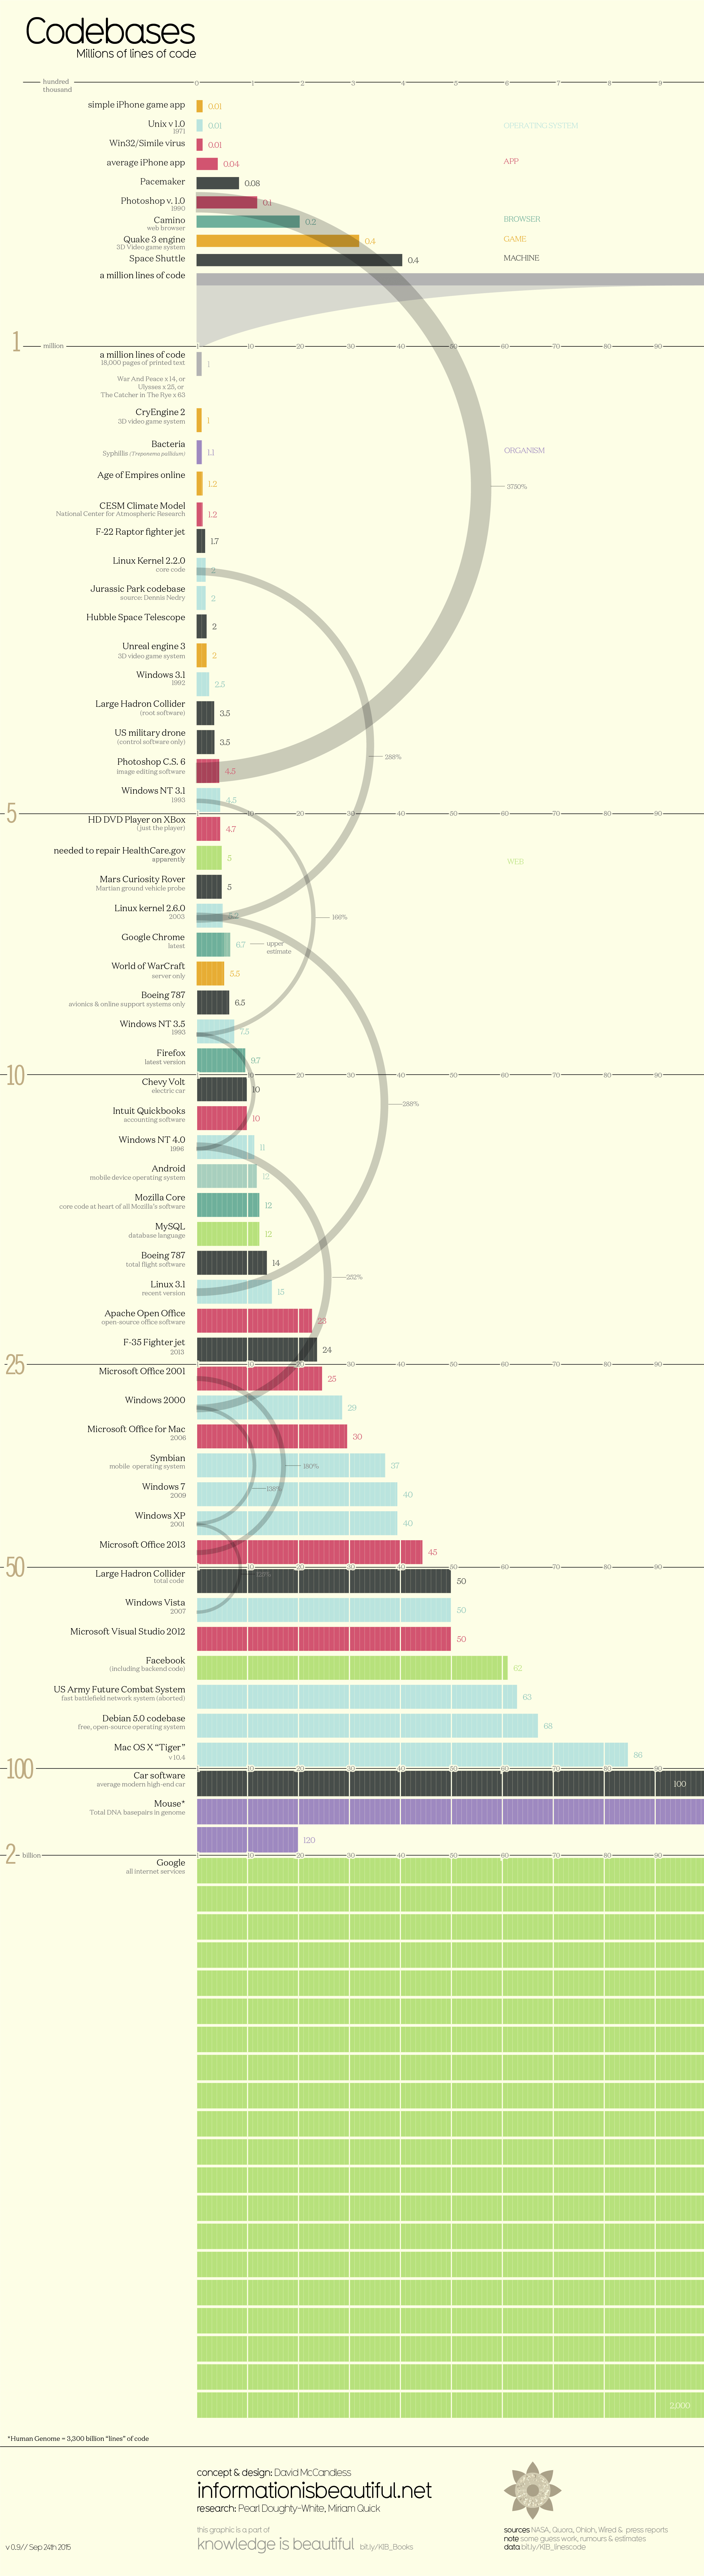
\includegraphics[angle=90,scale=0.05]{millions-lines-of-code-2015.png}
\centering
\begin{tikzpicture}
    \begin{axis}[
            ybar,
            bar width=6mm,
            width=\linewidth,
            height=.475\linewidth,
            %legend style={at={(0.5,1)},
            %    anchor=north,legend columns=-1},
            symbolic x coords={Pacemaker, Photoshop v1.0 (1990),
              Linux Kernel 2.2.0, Hubble Space Telescope, Windows 3.1 (1992), Photoshop C.S.6, Windows NT 3.1 (1993),
              Linux Kernel 2.6.0 (2003), Google Chrome, Firefox, Android, Boeing 787, Linux 3.1,
              Apache Open Office, Windows 2000 (2001), Windows XP (2001), Microsoft Office 2013, Facebook, 
              Debian 5.0 Codebase, Mac OS X Tiger v10.4},
            xtick=data,
            nodes near coords={\pgfmathprintnumber[precision=3]{\pgfplotspointmeta}},
            nodes near coords align={vertical},
            nodes near coords style={font=\scriptsize},
            %every node near coord/.append style={
            %  anchor=mid west,
            %  rotate=70
            %},
            axis x line*=bottom,% no top box x axis and no arrow tip (*)
            enlarge x limits=true,
            axis y line*=left,
            ymin=0,
            ymax=90,
            ylabel={Lignes de code (million)},
            y label style={font=\footnotesize},
            x tick label style={rotate=45, anchor=east, font=\footnotesize},
            y tick label style={font=\footnotesize},
            ymajorgrids, major grid style={draw=fourthcolor},
        ]
        \addplot[draw=secondcolor, fill=firstcolor] table[x=Name,y=Value]{\lineofcodes};
    \end{axis}
\end{tikzpicture}
\vspace{-4pt}
\caption{\label{fig:VI.5}Nombre de lignes de code de quelques applications connues (en million).}
\end{jazzfigure*}

\begin{gofurther}
\lightbf{Formation complémentaire}
\begin{itemize}\jazzitem
\item \href{https://pixees.fr/classcode/formations/module1/}{\#1 Module fondamental : découvrir la programmation créative}, \textsc{Class´Code}, Partie 2.4.
\end{itemize}

\vspace{2pt}
\lightbf{Articles}
\begin{itemize}\jazzitem
\item \href{http://images.math.cnrs.fr/Dis-papa-ou-maman-comment-arrivent-les-bugs-dans-le-monde-numerique}{Dis papa (ou maman) comment arrivent les \textit{bugs} dans le monde numérique}, Aurélien \textsc{Alvarez} et Thierry \textsc{Viéville}, \textsc{Images des mathématiques}, 2014.
\item \href{https://pixees.fr/comment-sont-entrees-mes-images-textes-donnees-dans-la-machine/}{Comment sont entrés mes images, textes, données dans la machine ?} avec l'article ci-dessus, le film les Sépas sur les \textit{bugs} et le jeu des pixels à travers le paravent en se passant bit à bit une image pour la reconstruire en aveugle.
\item \href{https://interstices.info/idee-recue-cest-la-faute-a-lordinateur/}{Idée reçue : c’est la faute à l’ordinateur !} Sylvie \textsc{Boldo}, \textsc{Interstices}, 19 février 2010.
\end{itemize}
\end{gofurther}

\subsubsection[Humains et langages]{Humains et langages}
\label{subsub:VI.2.2.2}

\begin{marginvideo}
	[\label{vid:VI.8}Choix d'un langage de programmation.]%
	\movie[width=\marginparwidth,showcontrols]%
		{
\includegraphics[width=\marginparwidth]{./Images/Pictograms/film-strip-dark-electric-blue.png}}%
		{./Videos/Chapter06/vidVI-08-human-languages-HD.mp4}%
	\launchvideo{./Videos/Chapter06/vidVI-08-human-languages-HD.mp4}
\end{marginvideo}

Il existe de très nombreux langages de programmation aux caractéristique différentes. Ce qu'il faut retenir, c'est qu'il est toujours possible de tout faire dans tous les langages de programmation. En revanche, cela ne sera pas toujours aussi facile, mais on peut utiliser n'importe quel langage de programmation pour écrire n'importe quel algorithme. 

On peut classer les langages par paradigmes de programmation :
\begin{itemize}
\item \emph{paradigme impératif}, le plus usuel et le plus proche du processeur ; on donne des ordres successivement, on fait des boucles, etc. Les exemples les plus traditionnels sont C\sidenote{Le langage C a été conçu pour programmer les premiers systèmes d'exploitation \textsc{Unix} au tout début de la décennie 1970.} et \textsc{Fortran} ;
\item \emph{paradigme fonctionnel}, on y considère les fonctions comme des objets à part entière qu'on peut passer à d'autres fonctions. C'est une vision un peu plus mathématique de la programmation. Les exemples de tels langages sont \textsc{Haskell} et \textsc{OCaml} ;
\item \emph{paradigme objet}, manière de faire de la programmation un peu plus générique, où effectivement on va pouvoir partager un certain nombre de fonctions entre des objets différents. Ce paradigme est très répandu actuellement et permet la réutilisation ou factorisation de code, gain de temps de développement. Les exemples sont \textsc{Java} et C++ ;
\item \emph{paradigme par contrainte} est plus une programmation logique dont un exemple est \textsc{Prolog}. Imaginons un calcul d'emploi du temps avec un certain nombre de contraintes : tel professeur n'est là que lundi matin, telle salle ne peut faire que de l'informatique, etc. Toutes ces contraintes sont prises en compte et on obtient idéalement un emploi du temps correct pour tous les professeurs et toutes les salles.
\item \emph{paradigme évènementiel}, le plus utilisé pour les interfaces graphiques ou la robotique. Le programme ne va pas se dérouler point par point, mais réagir à un certain nombre de \textit{stimuli} de l'environnement : un clic de souris sur l'interface d'un programme ou le contact d'un robot avec un obstacle. 
\end{itemize}

Dans les faits, beaucoup de langages de programmation sont multi-paradigmes ; c'est le cas de C++, \textsc{Java} ou \textsc{Python}... Notons également qu'on peut interfacer les langages entre eux de manière à profiter des atouts des deux langages ; \textsc{Python} est typiquement riche de bibliothèques de ce type --- écrites en C ou C++ --- qui sont transparentes pour le programmeur.

Au final, choisir un langage de programmation est invariablement une question compliquée. Cela dépend de ce qu'on veut programmer, de ce qu'on a l'habitude de faire et dans quel cadre.
\begin{itemize}\jazzitem
\item Quel paradigme de programmation ?
\item Quelles interfaces avec d'autres développements ? Souvent, le programme n'est qu'un morceau de projet plus conséquent et le « choix » s'avère imposé.
\item Quelles bibliothèques de support ? Pour une interface graphique, l'option adoptée peut être guidé par l'existence de bibliothèques graphiques ayant fait leur preuve.
\item Quelle connaissance préalable du langage ? A-t-on déjà de l’expérience dans un langage donné pour aller plus vite dans le développement ?
\item Quelle aide ou tutorat est mobilisable ? Peut-on solliciter son entourage pour avancer plus rapidement ?
\end{itemize}

\begin{gofurther}
\lightbf{Articles}
\begin{itemize}\jazzitem
\item Une définition des \href{https://fr.wikipedia.org/wiki/Paradigme_(programmation)}{paradigmes de programmation}, \textsc{Wikipédia}.
\item \href{https://interstices.info/bjarne-stroustrup-le-pere-de-c-un-langage-qui-a-de-la-classe/}{Bjarne \textsc{Stroustrup} : le père de C++, un langage qui a de la classe}, Pierre \textsc{Vandeginste}, \textsc{Interstices}, 15 juin 2004.
\item \href{https://interstices.info/la-programmation-par-contraintes/}{La programmation par contraintes}, Étienne \textsc{Parizot}, Sylvain \textsc{Soliman} et François \textsc{Fages}, \textsc{Interstices}, 24 février 2004.
\item \href{https://interstices.info/programmation-des-echecs-et-dautres-jeux/}{Programmation des échecs et d’autres jeux}, Olivier \textsc{Teytaud}, Interstices, 26 novembre 2012.
\end{itemize}

\vspace{2pt}
\lightbf{Vidéo}
\begin{itemize}\jazzitem
\item \href{https://www.canal-u.tv/video/inria/premiers_principes_des_langages_de_programmation.6473}{Premiers principes des langages de programmation}, cours introductif par Gilles \textsc{Dowek} à destination des professeurs des lycées ISN, CanalU (collection \textsc{Inria} Science Info Lycée Profs, (90 mn), 2010.
\end{itemize}

\vspace{2pt}
\lightbf{Site de programmation Interactive}
\begin{itemize}\jazzitem
\item \url{http://pythontutor.com/} est un outil en ligne qui n'est pas seulement dédié à \textsc{Python} comme son nom l'indique mais aussi à \textsc{JavaScript} : il permet d'écrire du code et de visualiser le résultat, ce qui peut aider à comprendre la programmation.
\end{itemize}

\end{gofurther}



%----------
\section[Que faire de ces ressources ? Quiz]{Que faire de ces ressources ? Autoévaluation}
\label{sec:VI.5}

Le questionnaire\caution[t]<firstcolor>{%
La présentation des quiz du document\linebreak suit plus ou moins celle de la platefor\-me \textsc{Fun-Mooc}. La fonctionnalité manquante --- pas encore implémentée dans l'extension de style \LaTeX{} usitée --- est relative à la comptabilisation des points et à leur enregistrement. Aussi, il appartient au lecteur de jouer le jeu dans l'auto\-évaluation de ses connaissances.}{Note de la rédaction}
à choix multiple%
\parnote{De manière traditionnelle en \textsc{Ihm}, lorsqu'une seule réponse est correcte, les propositions sont précédées d'un cercle à cocher (\emph{radio button}) ; en revanche, dans le cas de plusieurs solutions possibles, il s'agit de carrés (\emph{check box}). En outre, après validation des réponses (« Vérifier »), leur explication s'affiche en marge ou infobulle (« Afficher la réponse »).}
--- QCM --- à suivre clôture le présent chapitre \qnameref{chap:VI} et correspond à chaque sujet abordé.
\parnotes

\vspace{6pt}

\begin{quiz}[title={Décomposition en tâches}]
\vspace{-\baselineskip}
\begin{quizquestion*}[b]{2}{1,3,4}{Tâches élémentaires}
<L'ordinateur étant bête, il ne sait faire que des tâches très simples. C'est donc à nous, humains intelligents, de faire le travail de découpage.>
Pourquoi doit-on découper une tâche en tâches élémentaires ?
\points{1}
	\mcqproposal{Parce que ça nous embête.}
	\mcqproposal{Parce que l'ordinateur ne sait, par essence, exécuter que des tâches élémentaires.}
	\mcqproposal{Parce que c'est drôle.}
	\mcqproposal{Parce que l'ordinateur qui comprend tout veut vérifier qu'on sait le faire aussi.}
\end{quizquestion*}

\vfill\pagebreak

%\sidegraphic{\includegraphics[width=\linewidth]{arbre-genealogique.png}}% WORKS NO MORE! WHY?
%\afterpage{
\marginnote{\includegraphics[width=\linewidth]{arbre-genealogique.png}}
%}%
\begin{quizquestion*}<tooltip>[b]{4}{1,2,3,5,6,7}{Arbre généalogique}
<Les flèches vont du parent à l'enfant. Il y a donc une flèche de mon grand-père à mon parent, puis de mon parent à moi-même. Je dois donc suivre (descendre) deux flèches pour aller de mon grand-père à moi-même.>
\points{1}
Prenons un graphe bien connu : l'arbre généalogique. Les nœuds sont les personnes et il y a une flèche d'un parent à un enfant. Que dois-je faire pour aller de mon grand-père à moi-même ?
	\mcqproposal{Rester sur le nœud.}
	\mcqproposal{Descendre une flèche.}
	\mcqproposal{Remonter une flèche.}
	\mcqproposal{Descendre deux flèches.}
	\mcqproposal{Remonter deux flèches.}
	\mcqproposal{Descendre puis remonter une flèche.}
	\mcqproposal{Remonter puis descendre une flèche.}
\end{quizquestion*}
\end{quiz}


\begin{quiz}[title={Notion de variable}]
\vspace{-\baselineskip}
\begin{quizquestion}[b]{1,2,4}{3}{Utilité des variables}
<Les variables sont faites pour stocker tous types de valeurs : des entiers pour compter ou des valeurs plus complexes. Elles peuvent aussi permettre d'accéder à des endroits dans la mémoire. Elles permettent de stocker un morceau de musique (dans un certain format), mais pas directement de le faire jouer à un ordinateur.>
À quoi peut servir une variable ?
\points{1}
	\mcqproposal{À stocker la valeur d'un compteur.}
	\mcqproposal{À stocker une valeur ou le résultat d'un calcul.}
	\mcqproposal{À jouer de la musique.}
	\mcqproposal{À donner accès à un espace mémoire.}
\end{quizquestion}
\end{quiz}


\begin{quiz}[title={Instructions élémentaires}]
\vspace{-\baselineskip}
\begin{quizquestion*}[b]{4}{1,2,3}{Algorithme simple (I)}
<La valeur de \texttt{i} est initialisée à \texttt{2}. Elle n'est donc pas strictement négative. Il faut donc entrer dans la partie « sinon » du test. On soustrait donc \texttt{1} à \texttt{i} qui vaut au final \texttt{1}.>
Voici un algorithme simple à exécuter. Quelle est la valeur de \texttt{i} ?
\begin{lstlisting}[style=lstalgostyle]
i ← 2;
Si i < 0 Alors
  i ← i + 1;
Sinon
  i ← i - 1;
FinSi
\end{lstlisting}
\points{1}
	\mcqproposal{\texttt{i} vaut \texttt{2}.}
	\mcqproposal{\texttt{i} vaut \texttt{-1}.}
	\mcqproposal{\texttt{i} vaut \texttt{3}.}
	\mcqproposal{\texttt{i} vaut \texttt{1}.}
%	\mcqproposal{\texttt{i} vaut \texttt{0}.}
\end{quizquestion*}

\vfill\pagebreak

\begin{quizquestion*}[b]{4}{1,2,3,5}{Algorithme simple (II)}
<La boucle « \texttt{Pour} » va s'exécuter 6 fois (\texttt{i=0}, \texttt{i=1}, ... , \texttt{i=5}). À chaque tour de boucle, on ajoute \texttt{1} à \texttt{x}, donc \texttt{x} vaudra \texttt{6}.
Pour calculer \texttt{y}, on regarde en plus la valeur de \texttt{i} à chaque tour. Cela donne les valeurs successives : \texttt{y=0}, puis \texttt{i=0} et \texttt{y=0+0=0}, puis \texttt{i=1} et \texttt{y=0+1=1}, puis \texttt{i=2} et \texttt{y=1+2=3}, puis \texttt{i=3} et \texttt{y=3+3=6}, puis \texttt{i=4} et \texttt{y=6+4=10} et enfin \texttt{i=5} et \texttt{y=10+5=15}.>
\points{1}
Voici un algorithme simple à exécuter. Quelles sont les valeurs respectives de \texttt{x} et de \texttt{y} ?	
\begin{lstlisting}[style=lstalgostyle]
x ← 0; y ← 0;
Pour i de 0 à 5 inclus Faire
  x ← x + 1;
  y ← y + i;
FinPour
\end{lstlisting}
  \mcqproposal{\texttt{x = 5} et \texttt{y = 16}.}
  \mcqproposal{\texttt{x = 6} et \texttt{y = 12}.}
  \mcqproposal{\texttt{x = 7} et \texttt{y = 18}.}
  \mcqproposal{\texttt{x = 6} et \texttt{y = 15}.}
  \mcqproposal{\texttt{x = 5} et \texttt{y = 14}.}
\end{quizquestion*}

\begin{quizquestion}[c]{2,3,5,6}{1,4,7}{Boucles et algoritmique}
<La boucle « \texttt{Tant que} » peut ne jamais se terminer.
Deux différents algorithmes peuvent calculer la même chose. On préfère en général le plus rapide, mais il est parfois beaucoup plus compliqué !
Un tableau est une structure de données permettant un traitement homogène des données, étant donc supposées de même type (même si certains langages de programmation autorisent les listes hétérogènes, nous ne sommes qu'en algorithmique pour l'instant). Il est impossible de regarder toutes les cases en même temps (il peut y en avoir des millions). En programmation objet quand on mélange des éléments de types différents, du coup, le tableau peut être considéré comme un tableau d'objets.
On peut transformer une boucle « \texttt{Pour} » en une boucle « \texttt{Tant que} ». Par exemple,
« \texttt{Pour i de 0 à 100 Faire ... FinPour} » deviendrait « \texttt{i ← 0; TantQue i ≤ 100 Faire ... FinTantQue} ».
L'affectation permet de modifier une valeur, sans forcément se soucier de la valeur précédente.>
\points{1}
Sélectionnez les affirmations vraies. Il peut y en avoir plusieurs !
  \mcqproposal{Une boucle « \texttt{Tant que} » se termine toujours.}
  \mcqproposal{On peut avoir deux algorithmes différents pour la même chose.}
  \mcqproposal{Un tableau, au niveau algorithmique, doit être composé de valeurs de même type (numérique par exemple).}
  \mcqproposal{Le processeur (unité centrale) d'un ordinateur usuel peut traiter toutes les cases d'un tableau en même temps.}
  \mcqproposal{La boucle « \texttt{Pour} » peut s'écrire avec une boucle « \texttt{Tant que} ».}
  \mcqproposal{L'affectation peut permettre d'augmenter une valeur.}
  \mcqproposal{L'affectation ne peut que permettre d'augmenter une valeur (et pas de la diminuer).}
\end{quizquestion}
\end{quiz}

\begin{quiz}[title={Culture algoritmique}]
\vspace{-\baselineskip}
\begin{quizquestion}<tooltip>[b]{1,3,4}{2,5}{Algorithmes}
<Les algorithmes sont une des fondations de l'informatique. De nombreux livres et sites Internet les décrivent. Des gens en inventent et vous pouvez aussi en inventer (soit pour faire de nouvelles choses, soit pour faire des choses connues plus rapidement).>
\points{1}
Sélectionnez les affirmations vraies. Il peut y en avoir plusieurs !
  \mcqproposal{Je peux en inventer.}
  \mcqproposal{C'est seulement sur Internet.}
  \mcqproposal{Je peux en trouver dans des livres.}
  \mcqproposal{Des gens en inventent des nouveaux.}
  \mcqproposal{Ça ne sert à rien.}
\end{quizquestion}
\end{quiz}

\begin{quiz}[title={Langage machine}]
\vspace{-\baselineskip}
\begin{quizquestion*}[b]{1}{2}{Écriture}
<L'assembleur est un langage de très bas niveau. Il peut bien sûr être écrit directement (comme les premiers compilateurs), mais c'est assez rébarbatif et sujet à erreurs.>
\points{1}
On peut écrire l'assembleur directement à la main.
  \mcqproposal{Vrai.}
  \mcqproposal{Faux.}
\end{quizquestion*}

\begin{quizquestion*}[b]{2}{1}{Praticité}
<L'assembleur est un langage de très bas niveau. Il peut bien sûr être écrit directement (comme les premiers compilateurs), mais c'est assez rébarbatif et sujet à erreurs.>
\points{1}
C'est pratique et simple d'écrire l'assembleur directement à la main.
  \mcqproposal{Vrai.}
  \mcqproposal{Faux.}
\end{quizquestion*}
\end{quiz}

\begin{quiz}[title={Compilation}]
\vspace{-\baselineskip}
\begin{quizquestion}[b]{1}{2}{Compilateurs}
<Les compilateurs peuvent détecter certaines erreurs (syntaxe, parfois type), mais pas toutes...
Ils transforment ce qu'écrivent les programmeurs en exécutable machine ou en assembleur. Ils ont ansi en valeur d'entrée le texte d'un autre programme.>
À propos des compilateurs. Que dire ?
\points{1}
  \mcqproposal{Ils permettent de détecter des erreurs simples.}
  \mcqproposal{Ils permettent de détecter toutes les erreurs.}
  \mcqproposal{Ils transforment un texte compréhensible par un humain en quelque chose compréhensible par l'ordinateur.}
  \mcqproposal{Ils sont des programmes qui prennent en entrée un programme.}
\end{quizquestion}
\end{quiz}

\begin{quiz}[title={{\itshape Bugs} et bogues}]
\vspace{-\baselineskip}
%\begin{quizquestion}[b]{2,3,5,7}{1,4,6}{Occurence des {\upshape bugs}}
\begin{quizquestion}[b]{2,3,5,6}{1,4}{Occurence des {\upshape bugs}}
<Beaucoup de possibilités de \textit{bugs} ! Personne n'est bête dans cette histoire, mais le manque de communication ou l'étourderie sont souvent responsables.>
\points{1}
Les \textit{bugs} arrivent parce que (bien sélectionner toutes les possibilités) :
  \mcqproposal{les programmeurs sont bêtes.}
  \mcqproposal{les programmeurs se sont trompés.}
  \mcqproposal{les programmeurs n'ont pas prévu un cas particulier.}
  \mcqproposal{l'ordinateur n'a pas obéi aux programmeurs.}
  \mcqproposal{les programmeurs ont bien fait ce qu'on leur a demandé, mais pas ce que l'on voulait.}
%  \mcqproposal{l'utilisateur est bête.}
  \mcqproposal{les programmeurs n'ont pas communiqué entre eux.}
\end{quizquestion}

Les questions à suivre concernent les ordres de grandeurs de taille de code. Quels sont-ils ?

\begin{quizquestion*}[b]{1}{2,3,4}{Premier programme}
<La taille du code explique aussi la présence de \textit{bugs} et, la difficulté à les corriger !>
\points{1}
  \mcqproposal{Moins de 100 lignes.}
  \mcqproposal{De 100 à 1\,000 lignes.}
  \mcqproposal{Quelques millions de lignes.}
  \mcqproposal{Quelques dizaines de millions de lignes.}
\end{quizquestion*}

%\begin{quizquestion*}[b]{3}{1,2,4}{Sonde spatiale Hubble}
%<La taille du code explique aussi la présence de \textit{bugs} et, la difficulté à les corriger !>
%\points{1}
%  \mcqproposal{Moins de 100 lignes.}
%  \mcqproposal{De 100 à 1\,000 lignes.}
%  \mcqproposal{Quelques millions de lignes.}
%  \mcqproposal{Quelques dizaines de millions de lignes.}
%\end{quizquestion*}

\begin{quizquestion*}[b]{2}{1,3,4}{Premier projet ou jeu}
<La taille du code explique aussi la présence de \textit{bugs} et, la difficulté à les corriger !>
\points{1}
  \mcqproposal{Moins de 100 lignes.}
  \mcqproposal{De 100 à 1\,000 lignes.}
  \mcqproposal{Quelques millions de lignes.}
  \mcqproposal{Quelques dizaines de millions de lignes.}
\end{quizquestion*}

\begin{quizquestion*}[b]{4}{1,2,3}{{\scshape Facebook}}
<La taille du code explique aussi la présence de \textit{bugs} et, la difficulté à les corriger !>
\points{1}
  \mcqproposal{Moins de 100 lignes.}
  \mcqproposal{De 100 à 1\,000 lignes.}
  \mcqproposal{Quelques millions de lignes.}
  \mcqproposal{Quelques dizaines de millions de lignes.}
\end{quizquestion*}

\begin{quizquestion*}[b]{3}{1,2,4}{{\scshape Boeing 787}}
<La taille du code explique aussi la présence de \textit{bugs} et, la difficulté à les corriger !>
\points{1}
  \mcqproposal{Moins de 100 lignes.}
  \mcqproposal{De 100 à 1\,000 lignes.}
  \mcqproposal{Quelques millions de lignes.}
  \mcqproposal{Quelques dizaines de millions de lignes.}
\end{quizquestion*}
\end{quiz}

\begin{quiz}[title={Langage de programmation}]
\vspace{-\baselineskip}
\begin{quizquestion}[b]{1,3,5}{2,4}{Choix des langages}
<Les langages de programmation pren\-nent naissance et se développent suivant les besoins et l'apparition de nouvelles idées pour programmer mieux ou plus facilement. Ils sont plus ou moins adaptés à l'application voulue, même si on peut toujours tout faire.>
Pourquoi y-a-t-il plusieurs langages de programmation ?
\points{1}
  \mcqproposal{Parce que les programmeurs ont des préférences.}
  \mcqproposal{Parce que cela crée plus d'emplois de programmeur.}
  \mcqproposal{Parce que certains langages sont plus adaptés à résoudre certains problèmes.}
  \mcqproposal{Pour que ce soit difficile d'échanger des bouts de programme.}
  \mcqproposal{Parce que de nouveaux paradigmes (types de programmation) sont apparus.}
\end{quizquestion}

\begin{quizquestion}[b]{1,3,4,6}{2,5,7}{Paradigmes de programmation}
<Il existe des langages impératif, fonctionnel, objet ou/et événementiel. Par contre, aucun langage n'utilise le paradigme du clavier ou de la cuisine (enfin un type de programmation qui nourrit !).>
Lesquels sont des paradigmes de programmation ?
\points{1}
  \mcqproposal{Objet.}
  \mcqproposal{Cuisine.}
  \mcqproposal{Fonctionnel.}
  \mcqproposal{Événementiel.}
  \mcqproposal{Clavier.}
  \mcqproposal{Impératif.}
  \mcqproposal{Utile.}
\end{quizquestion}

\begin{quizquestion*}[b]{2}{1,3,4}{Programme en C}
<À essayer !>
Complétez le programme suivant en C. Le but est de chercher la valeur 17 dans un tableau et de le remplacer par 0.
On suppose avoir un tableau \texttt{t} de taille \texttt{N}. On peut alors écrire :\\
\points{1}
\texttt{for (i=0;i < N;i++) \{}\\
\hspace*{1.5ex}\texttt{????} $\leftarrow$ compléter par une des propositions ci-dessous\\
\texttt{t[i] = 0; \}}
  \mcqproposal{\texttt{while (t[i]==17)}}
  \mcqproposal{\texttt{if (t[i]==17)}}
  \mcqproposal{\texttt{t[i]=17}}
  \mcqproposal{\texttt{t[0]==17}}
\end{quizquestion*}
\end{quiz}



\vfill\pagebreak\thispagestyle{empty}












